\documentclass[12pt,addpoints]{evalua}
\grado{6$^\circ$ de Primaria}
\cicloescolar{2024-2025}
\materia{Matemáticas}
\unidad{}
\title{Examen General}
\aprendizajes{\tiny%
% \item Estudio de los números.
\item Expresa oralmente la sucesión numérica hasta billones, en español y hasta donde sea posible, en su lengua materna, de manera ascendente y descendente a partir de un número natural dado. Ordena, lee y escribe números naturales de más de nueve cifras e interpreta números decimales en diferentes contextos. Identifica semejanzas y diferencias entre el sistema de numeración decimal y otros sistemas como el maya y el romano\\[-1.5em]
	% \item Suma y resta, su relación como operaciones inversas.
	\item A partir de situaciones problemáticas vinculadas a diferentes contextos, suma y resta números decimales y fracciones con diferentes denominadores.\\[-1.5em]
	% \item Multiplicación y división, su relación como operaciones inversas.
	\item Resuelve situaciones problemáticas vinculadas a diferentes contextos que implican dividir números decimales entre naturales. También, dividir números fraccionarios entre números naturales.\\[-1.5em]
	% \item Relaciones de proporcionalidad.
	\item A partir de situaciones problemáticas de proporcionalidad vinculadas a diferentes contextos, determina valores faltantes en las que en ocasiones se conoce el valor unitario y en otras no.\\[-1.5em]
	% \item Ubicación espacial.
	\item Lee, interpreta y elabora planos para comunicar la ubicación de seres vivos y objetos.\\[-1.5em]
	% \item Figuras y cuerpos geométricos y sus características.
	\item Explora y reconoce las características del cilindro y cono; anticipa y comprueba desarrollos planos que permiten construirlos.\\[-1.5em]
	% \item Perímetro, área y noción de volumen.
	\item Resuelve situaciones problemáticas que implican calcular el perímetro y área de figuras compuestas por triángulos y cuadriláteros. Resuelve problemas que implican construir, estimar y comparar el volumen de cuerpos y prismas rectos rectangulares mediante el conteo de cubos, y reconoce que existen diferentes cuerpos con el mismo volumen.\\[-1.5em]
	% \item Organización e interpretación de datos.
	\item Interpreta información cuantitativa y cualitativa contenida en tablas, gráficas de barras y circulares para responder preguntas vinculadas a diferentes contextos; construye gráficas de barras. Genera y organiza datos, determina la moda, la media aritmética y el rango para responder preguntas vinculadas a diferentes contextos.\\[-1.5em]
	% \item Nociones de probabilidad.
	\item Clasifica eventos de diversos contextos utilizando términos como seguro, imposible, probable, muy probable o poco probable que sucedan.
}
\author{Prof.: Julio César Melchor Pinto}
\begin{document}
\afterpage{\blankpage}%
\begin{multicols}{2}
	\tableofcontents
\end{multicols}
\begin{questions}

   \addcontentsline{toc}{section}{Unidad 1}
	\section*{Unidad 1}

	\addcontentsline{toc}{subsection}{Sumas y restas}
	\subsection*{Sumas y restas}

	% \addcontentsline{toc}{subsubsection}{Sumas 1}
	% \subsubsection*{Sumas 1}
	% \addcontentsline{toc}{subsubsection}{Sumas 2}
	% \subsubsection*{Sumas 2}
	% \addcontentsline{toc}{subsubsection}{Restas 1}
	% \subsubsection*{Restas 1}
	% \addcontentsline{toc}{subsubsection}{Restas 2}
	% \subsubsection*{Restas 2}
   \question[4]{Realiza las siguientes sumas y restas:

   \begin{multicols}{4}
      \begin{parts}
         \part
         \ifprintanswers{\opadd[hfactor=decimal,resultstyle=\color{red},carryadd=true]{17}{18}}
         \else{\opadd[hfactor=decimal,resultstyle=\color{white},carryadd=false]{17}{18}\\[0.5cm]}\fi


         \part \ifprintanswers{   \opsub[hfactor=decimal,resultstyle=\color{red},carryadd=true,carrysub=true]{706}{589}}
         \else{            \opsub[hfactor=decimal,resultstyle=\color{white},carryadd=false,carrysub=false]{706}{589}\\[0.5cm]}\fi

         \part
         \ifprintanswers{\opadd[hfactor=decimal,resultstyle=\color{red},carryadd=true]{1155}{893}}
         \else{\opadd[hfactor=decimal,resultstyle=\color{white},carryadd=false]{1155}{893}\\[0.5cm]}\fi


         \part \ifprintanswers{   \opsub[hfactor=decimal,resultstyle=\color{red},carryadd=true,carrysub=true]{3004}{1242}}
         \else{            \opsub[hfactor=decimal,resultstyle=\color{white},carryadd=false,carrysub=false]{3004}{1242}\\[0.5cm]}\fi

         % \part
         % \ifprintanswers{\opadd[hfactor=decimal,resultstyle=\color{red},carryadd=true]{26}{19}}
         % \else{\opadd[hfactor=decimal,resultstyle=\color{white},carryadd=false]{26}{19}\\[0.5cm]}\fi


         % \part \ifprintanswers{   \opsub[hfactor=decimal,resultstyle=\color{red},carryadd=true,carrysub=true]{1600}{669}}
         % \else{            \opsub[hfactor=decimal,resultstyle=\color{white},carryadd=false,carrysub=false]{1600}{669}\\[0.5cm]}\fi

         % \part
         % \ifprintanswers{\opadd[hfactor=decimal,resultstyle=\color{red},carryadd=true]{2271}{1028}}
         % \else{\opadd[hfactor=decimal,resultstyle=\color{white},carryadd=false]{2271}{1028}\\[0.5cm]}\fi

         % \part \ifprintanswers{   \opsub[hfactor=decimal,resultstyle=\color{red},carryadd=true,carrysub=true]{4005}{2831}}
         % \else{            \opsub[hfactor=decimal,resultstyle=\color{white},carryadd=false,carrysub=false]{4005}{2831}\\[0.5cm]}\fi
      \end{parts}
   \end{multicols}
}
	% \addcontentsline{toc}{subsubsection}{Resolución de problemas}
	% \subsubsection*{Resolución de problemas}

	\question[3]{Resuelve los siguientes problemas sobre sumas, restas y multiplicaciones:

		\begin{multicols}{3}
			\begin{parts}
				% \part El total de mis compras es de 315 pesos, ¿cuánto dinero recibiré de cambio si pago con un billete de 500 pesos?

				% \begin{solutionbox}{1cm}
				% 	\opsub[style=text]{500}{315}
				% \end{solutionbox}

				\part Luis tiene ahorrado 257 pesos, si su abuelo le regala 360 pesos más, ¿cuánto dinero tiene en total Luis?

				\begin{solutionbox}{1cm}
					\opadd[style=text]{257}{360}
				\end{solutionbox}

				% \part Jorge está armando un rompecabezas de 500 piezas, si ha puesto 233 piezas, ¿cuántas piezas le faltan por poner a Jorge?

				% \begin{solutionbox}{1.2cm}
				% 	\opsub[style=text]{500}{233}
				% \end{solutionbox}

				\part Carlos mide 183 centímetros y es 8 centímetros más alto que Julio, ¿cuántos centímetros mide Julio?

				\begin{solutionbox}{1.2cm}
					\opsub[style=text]{183}{8}
				\end{solutionbox}

            \part Laura compró 28 paquetes de galletas, si cada paquete tiene 18 galletas. ¿Cuántas galletas tiene en total Laura?

            \begin{solutionbox}{1.5cm}
               \opmul[style=text]{28}{18}
            \end{solutionbox}
			\end{parts}
		\end{multicols}
	}



	\addcontentsline{toc}{subsection}{Multiplicaciones y divisiones}
	\subsection*{Multiplicaciones y divisiones}

	% \addcontentsline{toc}{subsubsection}{Multiplicaciones 1}
	% \subsubsection*{Multiplicaciones 1}
	% \addcontentsline{toc}{subsubsection}{Multiplicaciones 2}
	% \subsubsection*{Multiplicaciones 2}
   \question[4]{Realiza las siguientes multiplicaciones y divisiones:

   \begin{multicols}{4}
      \begin{parts}
         \part \ifprintanswers{\normalsize\opmul[hfactor=decimal,resultstyle=\color{red},displayintermediary=None]{314}{2} }
         \else{\opmul[hfactor=decimal,resultstyle=\color{white},displayintermediary=None]{314}{2}}\\[2em]\fi

         \part \ifprintanswers{\opidiv[resultstyle=\color{red},remainderstyle.1=\color{blue!100!white}]{23}{6}} 
         \else{           $6 \overline{) \ 23\ }$} \\[2em]
         \fi

         \part \ifprintanswers{\normalsize\opmul[hfactor=decimal,resultstyle=\color{red},displayintermediary=all]{283}{44} }
         \else{\opmul[hfactor=decimal,resultstyle=\color{white},displayintermediary=None]{283}{44}}\\[2em]\fi

         \part \ifprintanswers{\opidiv[resultstyle=\color{red},remainderstyle.3=\color{blue!100!white}]{4032}{8}} 
         \else{           $8 \overline{) \ 4032\ }$} \\[2em]
         \fi
         % \part \ifprintanswers{\normalsize\opmul[hfactor=decimal,resultstyle=\color{red},displayintermediary=None]{2781}{5} }
         % \else{\opmul[hfactor=decimal,resultstyle=\color{white},displayintermediary=None]{2781}{5}}\\[2em]\fi

         % \part \ifprintanswers{\normalsize\opmul[hfactor=decimal,resultstyle=\color{red},displayintermediary=all]{3914}{106} }
         % \else{\opmul[hfactor=decimal,resultstyle=\color{white},displayintermediary=None]{3914}{106}}\\[2em]\fi

         % \part \ifprintanswers{\normalsize\opmul[hfactor=decimal,resultstyle=\color{red},displayintermediary=all]{255}{24} }
         % \else{\opmul[hfactor=decimal,resultstyle=\color{white},displayintermediary=None]{255}{24}}\\[2em]\fi

         % \part \ifprintanswers{\normalsize\opmul[hfactor=decimal,resultstyle=\color{red},displayintermediary=all]{3533}{29} }
         % \else{\opmul[hfactor=decimal,resultstyle=\color{white},displayintermediary=None]{3533}{29}}\\[2em]\fi
      \end{parts}
   \end{multicols}
}


% \addcontentsline{toc}{subsubsection}{Divisiones 1}
	% \subsubsection*{Divisiones 1}
	% \addcontentsline{toc}{subsubsection}{Divisiones 2}
	% \subsubsection*{Divisiones 2}
% \addcontentsline{toc}{subsection}{División}
% \subsection*{División}

% \question[4]{Calcula el {\color{red}cociente} y {\color{blue} residuo} de las siguientes divisiones de números enteros:

%    \begin{multicols}{4}
%       \begin{parts}
        
%          \part \ifprintanswers{\opidiv[resultstyle=\color{red},remainderstyle.2=\color{blue!100!white}]{200}{3}} 
%          \else{           $3 \overline{) \ 200\ }$} \\[2em]
%          \fi

%          % \part \ifprintanswers{\opidiv[resultstyle=\color{red},remainderstyle.2=\color{blue!100!white}]{99}{8}} 
%          % \else{           $8 \overline{) \ 99\ }$} \\[4em]
%          % \fi

%          % \part \ifprintanswers{\opidiv[resultstyle=\color{red},remainderstyle.2=\color{blue!100!white}]{283}{6}} 
%          % \else{           $6 \overline{) \ 283\ }$} \\[4em]
%          % \fi

%          \part \ifprintanswers{\opidiv[resultstyle=\color{red},remainderstyle.3=\color{blue!100!white}]{4032}{8}} 
%          \else{           $8 \overline{) \ 4032\ }$} \\[2em]
%          \fi

%          % \part \ifprintanswers{\opidiv[resultstyle=\color{red},remainderstyle.2=\color{blue!100!white}]{644}{8}} 
%          % \else{           $8 \overline{) \ 644\ }$} \\[4em]
%          % \fi

%          % \part \ifprintanswers{\opidiv[resultstyle=\color{red},remainderstyle.2=\color{blue!100!white}]{656}{7}} 
%          % \else{           $7 \overline{) \ 656\ }$} \\[4em]
%          % \fi

%          \part \ifprintanswers{\opidiv[resultstyle=\color{red},remainderstyle.3=\color{blue!100!white}]{2303}{7}} 
%          \else{           $7 \overline{) \ 2303\ }$} \\[2em]
%          \fi
%       \end{parts}
%    \end{multicols}
% }
	






	\addcontentsline{toc}{subsection}{Números decimales}
	\subsection*{Números decimales}
	% \addcontentsline{toc}{subsubsection}{Posición decimal y notación desarrollada}
	% \subsubsection*{Posición decimal y notación desarrollada}


	\question[2]{Señala la opción que responda correctamente a cada una de las siguientes preguntas:

		\begin{multicols}{2}
			\begin{parts}
				% \part En el número 1.829, ¿qué número ocupa la posición de las centésimas?

				% \begin{oneparcheckboxes}
				% 	\choice 1 \CorrectChoice 2 \choice 6 \choice 8 \choice 9
				% \end{oneparcheckboxes}

				\part En el número 2.087, ¿qué número ocupa la posición de las décimas?

				\begin{oneparcheckboxes}
					\CorrectChoice 0 \choice 2 \choice 7 \choice 8 \choice 9
				\end{oneparcheckboxes}

				\part En el número 5.928, ¿qué número ocupa la posición de las décimas?

				\begin{oneparcheckboxes}
					\choice 5 \choice 2 \choice 6 \choice 8 \CorrectChoice 9
				\end{oneparcheckboxes}

				\part En el número 3.284, ¿qué número ocupa la posición de las milésimas?

				\begin{oneparcheckboxes}
					\choice 2 \choice 3 \CorrectChoice 4  \choice 8 \choice 9
				\end{oneparcheckboxes}

				\part En el número 1.285, ¿qué número ocupa la posición de las décimas?

				\begin{oneparcheckboxes}
					\choice 1 \CorrectChoice 2 \choice 5 \choice 8 \choice 9
				\end{oneparcheckboxes}

				% \part En el número 1.823, ¿qué número ocupa la posición de las milésimas?

				% \begin{oneparcheckboxes}
				% 	\choice 1 \choice 2 \CorrectChoice 3 \choice 6 \choice 8
				% \end{oneparcheckboxes}
			\end{parts}
		\end{multicols}
	}

	% \addcontentsline{toc}{subsubsection}{Decimales en la recta numérica}
	% \subsubsection*{Decimales en la recta numérica}

	\question[2]{Escribe en el recuadro el número decimal que representa el punto en la recta numérica de cada imagen:

		\begin{multicols}{2}
			\begin{parts}
				\part 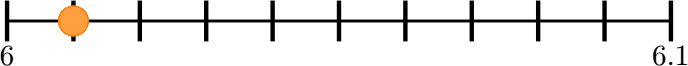
\includegraphics[width=180px]{../images/recta_num_6.01.png}  \hfill \fillin[\fbox{6.01}][0in] \\
				% \part 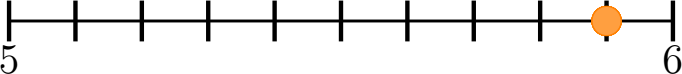
\includegraphics[width=180px]{../images/recta_num_5.9.png}   \hfill \fillin[\fbox{5.9 }][0in] \\
				% \part 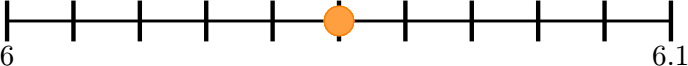
\includegraphics[width=180px]{../images/recta_num_6.05.png}  \hfill \fillin[\fbox{6.05}][0in] \\
				\part 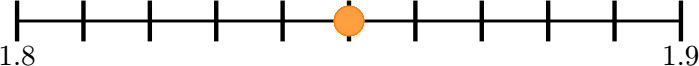
\includegraphics[width=180px]{../images/recta_num_1.85.png}  \hfill \fillin[\fbox{1.85}][0in] \\
				% \part 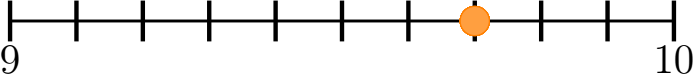
\includegraphics[width=180px]{../images/recta_num_9.7.png}   \hfill \fillin[\fbox{9.7 }][0in] \\
				\part 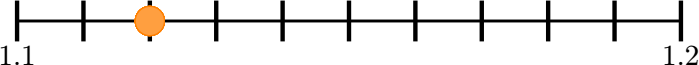
\includegraphics[width=180px]{../images/recta_num_1.12.png}  \hfill \fillin[\fbox{1.12}][0in] \\
				\part 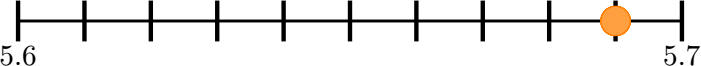
\includegraphics[width=180px]{../images/recta_num_5.69.png}  \hfill \fillin[\fbox{5.69}][0in] \\
				% \part 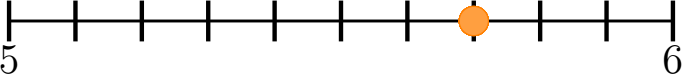
\includegraphics[width=180px]{../images/recta_num_5.7.png}   \hfill \fillin[\fbox{5.7 }][0in] \\
				% \part 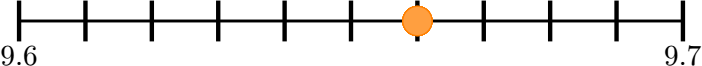
\includegraphics[width=180px]{../images/recta_num_9.66.png}  \hfill \fillin[\fbox{9.66}][0in] \\
				% \part 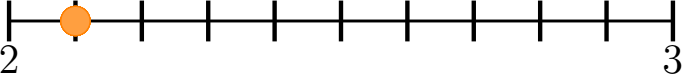
\includegraphics[width=180px]{../images/recta_num_2.1.png}   \hfill \fillin[\fbox{2.1 }][0in] \\
			\end{parts}
		\end{multicols}
	}

	% \addcontentsline{toc}{subsubsection}{Nombre de decimales}
	% \subsubsection*{Nombre de decimales}
	\question[2]{Escribe los siguientes números

		\begin{multicols}{2}
			\begin{parts}\normalsize
				% \part Catorce enteros diecinueve centésimos 	\hfill \fillin[14.19][1.2cm]
				\part Cuatro enteros once diez milésimos 		\hfill \fillin[4.0011][1.2cm]
				% \part Seis enteros setenta y dos centésimos 	\hfill \fillin[6.72][1.2cm]
				% \part Siete enteros novecientos tres milésimos 	\hfill \fillin[7.903][1.2cm]
				% \part Seis enteros doscientos trece milésimos 	\hfill \fillin[6.213][1.2cm]
				% \part Cincuenta enteros cinco décimos 			\hfill \fillin[50.5][1.2cm]
				\part Nueve enteros cuatro centésimos 			\hfill \fillin[9.04][1.2cm]
				% \part Cuatro enteros setecientos doce milésimos \hfill \fillin[4.712][1.2cm]
				\part Seis mil catorce diez milésimos 			\hfill \fillin[0.6014][1.2cm]
				% \part Nueve enteros once centésimos 			\hfill \fillin[9.11][1.2cm]
				% \part Cuarenta enteros cuatro centésimos 		\hfill \fillin[40.04][1.2cm]
				% \part Dieciocho enteros siete décimos 			\hfill \fillin[18.7][1.2cm]
				% \part Veinte enteros tres décimos 				\hfill \fillin[20.3][1.2cm]
				\part Cuatro enteros ciento dos diez milésimos 	\hfill \fillin[4.0102][1.2cm]
				% \part Ocho enteros trece diez milésimos 		\hfill \fillin[8.0013][1.2cm]
			\end{parts}
		\end{multicols}
	}

	

	%%% \addcontentsline{toc}{subsubsection}{Comparación de decimales}
	%%% \subsubsection*{Comparación de decimales}
	%%% \addcontentsline{toc}{subsubsection}{Redondeo de decimales}
	%%% \subsubsection*{Redondeo de decimales}

	\question[2]{\textbf{Redondea} los siguientes números decimales como se pide:

		\begin{multicols}{2}
			\begin{parts}\normalsize
				\part $8.0375 $ a la milésima más cercana       \hfill \fillin[$8.038 $][1.2cm]
				% \part $3.09628$ a la diez milésima más cercana  \hfill \fillin[$3.0963$][1.2cm]
				% \part $3.28   $ a la décima más cercana         \hfill \fillin[$3.3   $][1.2cm]
				% \part $5.308  $ a la centésima más cercana      \hfill \fillin[$5.31  $][1.2cm]
				% \part $8.57   $ a la décima más cercana         \hfill \fillin[$8.6   $][1.2cm]
				% \part $7.229  $ a la décima más cercana         \hfill \fillin[$7.2   $][1.2cm]
				% \part $9.85713$ a la milésima más cercana       \hfill \fillin[$9.857 $][1.2cm]
				% \part $6.12   $ a la décima más cercana         \hfill \fillin[$6.1   $][1.2cm]
				% \part $3.4952 $ a la milésima más cercana       \hfill \fillin[$3.495 $][1.2cm]
				% \part $2.52   $ a la décima más cercana         \hfill \fillin[$2.5   $][1.2cm]
				\part $6.28629$ a la diez milésima más cercana  \hfill \fillin[$6.2863$][1.2cm]
				\part $1.9286 $ a la milésima más cercana       \hfill \fillin[$1.929 $][1.2cm]
				% \part $4.27   $ a la décima más cercana         \hfill \fillin[$4.3   $][1.2cm]
				% \part $3.4025 $ a la décima más cercana         \hfill \fillin[$3.4   $][1.2cm]
				\part $5.03751$ a la milésima más cercana       \hfill \fillin[$5.038 $][1.2cm]
			\end{parts}
		\end{multicols}
	}

	\addcontentsline{toc}{subsection}{Operaciones con decimales}
	\subsection*{Operaciones con decimales}
	% \addcontentsline{toc}{subsubsection}{Suma de decimales}
	% \subsubsection*{Suma de decimales}

	
	% \addcontentsline{toc}{subsubsection}{Resta de decimales}
	% \subsubsection*{Resta de decimales}

	
	% \addcontentsline{toc}{subsubsection}{Multiplicación de decimales}
	% \subsubsection*{Multiplicación de decimales}



	%%% \addcontentsline{toc}{subsubsection}{División de decimales}
	%%% \subsubsection*{División de decimales}

   \question[6]{Realiza las siguientes sumas, restas, multiplicaciones y divisiones con números decimales:

   \begin{multicols}{3}
      \begin{parts}
         \part \ifprintanswers{   \opsub[hfactor=decimal,resultstyle=\color{red},carryadd=true,carrysub=true]{6.231}{2.188} }
         \else{            \opsub[hfactor=decimal,resultstyle=\color{white},carryadd=false,carrysub=false]{6.231}{2.188}\\[0.5cm] }
         \fi
      
         \part \ifprintanswers{\normalsize\opmul[hfactor=decimal,resultstyle=\color{red},displayintermediary=all]{5.3}{1.6} }
         \else{\opmul[hfactor=decimal,resultstyle=\color{white},displayintermediary=None]{5.3}{1.6}}\\[2em]\fi


         \part \ifprintanswers{   \opadd[hfactor=decimal,resultstyle=\color{red},carryadd=true,carrysub=false]{18.03}{7.45} }
         \else{            \opadd[hfactor=decimal,resultstyle=\color{white},carryadd=false,carrysub=false]{18.03}{7.45}\\[0.5cm] }
         \fi

         \part \ifprintanswers{\opdiv[shiftdecimalsep=divisor,strikedecimalsepsymbol=\hspace{-2.5pt}\tiny\color{red!50!black}$\times$]{4.025}{2.3}} 
         \else{           $2.3 \overline{) \ 4.025\ }$} \\[0.5em]\fi


         \part \ifprintanswers{\normalsize\opmul[hfactor=decimal,resultstyle=\color{red},displayintermediary=all]{2.5}{2.3} }
         \else{\opmul[hfactor=decimal,resultstyle=\color{white},displayintermediary=None]{2.5}{2.3}}\\[2em]\fi
      
         \part \ifprintanswers{\opdiv[shiftdecimalsep=divisor,strikedecimalsepsymbol=\hspace{-2.5pt}\tiny\color{red!50!black}$\times$]{17.6}{3.2}} 
         \else{           $3.2 \overline{) \ 17.6\ }$} \\[2em]
         \fi
      \end{parts}
   \end{multicols}
}

	
	%%% \addcontentsline{toc}{subsubsection}{Resolución de problemas}
	%%% \subsubsection*{Resolución de problemas}

	\addcontentsline{toc}{subsection}{Números decimales a fracciones}
	\subsection*{Números decimales a fracciones}
	%%% \addcontentsline{toc}{subsubsection}{Ubicación en la recta numérica}
	%%% \subsubsection*{Ubicación en la recta numérica}


	% \addcontentsline{toc}{subsubsection}{Porcentajes a decimal}
	% \subsubsection*{Porcentajes a decimal}

	\question[2]{Escribe los siguientes porcentajes como números decimales:

		\begin{multicols}{4}
			\begin{parts}
				% \part $14\%=$ \fillin[\fbox{0.14}][0cm] \\
				% \part $73\%=$ \fillin[\fbox{0.73}][0cm] \\
				% \part $15\%=$ \fillin[\fbox{0.15}][0cm] \\
				% \part $85\%=$ \fillin[\fbox{0.85}][0cm] \\
				\part $91\%=$ \fillin[\fbox{0.91}][0cm] 
				\part $19\%=$ \fillin[\fbox{0.19}][0cm] 
				% \part $ 9\%=$ \fillin[\fbox{0.09}][0cm] \\
				\part $42\%=$ \fillin[\fbox{0.42}][0cm] 
				% \part $25\%=$ \fillin[\fbox{0.25}][0cm] \\
				% \part $ 3\%=$ \fillin[\fbox{0.03}][0cm] \\
				% \part $ 8\%=$ \fillin[\fbox{0.08}][0cm] \\
				\part $ 2\%=$ \fillin[\fbox{0.02}][0cm] 
			\end{parts}
		\end{multicols}
	}

	%%% \addcontentsline{toc}{subsubsection}{Operaciones con múltiplos de 10}
	%%% \subsubsection*{Operaciones con múltiplos de 10}


	% \addcontentsline{toc}{subsubsection}{Conversión de fracciones a decimales}
	% \subsubsection*{Conversión de fracciones a decimales}

	\question[2]{Convierte las siguientes fracciones a decimal:

		\begin{multicols}{4}
			\begin{parts}
				% \part $\dfrac{2}{9} =$   \fillin[\fbox{$0.\overline{2}$}][0cm]\\
				% \part $\dfrac{1}{4} =$   \fillin[\fbox{$0.25$}][0cm]\\
				% \part $\dfrac{2}{3} =$   \fillin[\fbox{$0.\overline{6}$}][0cm]\\
				% \part $\dfrac{7}{8} =$   \fillin[\fbox{$0.875$}][0cm]\\
				\part $\dfrac{1}{9} =$   \fillin[\fbox{$0.\overline{1}$}][0cm]
				\part $\dfrac{6}{8} =$   \fillin[\fbox{$0.75$}][0cm]
				% \part $\dfrac{7}{20}=$   \fillin[\fbox{$0.35$}][0cm]\\
				\part $\dfrac{5}{8} =$   \fillin[\fbox{$0.625$}][0cm]
				% \part $\dfrac{2}{10}=$   \fillin[\fbox{$0.2$}][0cm]\\
				\part $\dfrac{5}{6} =$   \fillin[\fbox{$0.8\overline{3}$}][0cm]
			\end{parts}
		\end{multicols}
	}

	% \addcontentsline{toc}{subsubsection}{Conversión de decimales a fracciones}
	% \subsubsection*{Conversión de decimales a fracciones}

	\question[2]{Convierte los siguientes números decimales a una fracción \textbf{simplificada} a su mínima expresión:

		\begin{multicols}{4}
			\begin{parts}
				\part $0.248=$ \fillin[\fbox{$\dfrac{31}{125}$}][0cm]
				% \part $0.46=$  \fillin[\fbox{$\dfrac{23}{50}$}][0cm]
				\part $0.24=$  \fillin[\fbox{$\dfrac{6}{25}$}][0cm]
				% \part $0.9=$   \fillin[\fbox{$\dfrac{9}{10}$}][0cm]
				\part $0.115=$ \fillin[\fbox{$\dfrac{23}{200}$}][0cm]
				\part $0.66=$  \fillin[\fbox{$\dfrac{33}{50}$}][0cm]
				% \part $0.56=$  \fillin[\fbox{$\dfrac{14}{25}$}][0cm]
				% \part $0.58=$  \fillin[\fbox{$\dfrac{29}{50}$}][0cm]
			\end{parts}
		\end{multicols}
	}

	\newpage
	\addcontentsline{toc}{section}{Unidad 2}
	\section*{Unidad 2}

	\addcontentsline{toc}{subsection}{Introducción a fracciones}
	\subsection*{Introducción a fracciones}
	% \addcontentsline{toc}{subsubsection}{Clasificación de fracciones}
	% \subsubsection*{Clasificación de fracciones}

	\question[2]{Escribe sobre la línea la clasificación de cada una de las fracciones: (\textit{propias, impropias o mixtas}):

		\begin{multicols}{3}
			\begin{parts}
				\part $\dfrac{5}{6}$   \fillin[Propia][1.5cm]     \\[0.5em]
				\part $5\dfrac{5}{11}$ \fillin[Mixta][1.5cm]      \\[0.5em]
				\part $\dfrac{13}{12}$   \fillin[Impropia][1.5cm] \\[0.5em]
				% \part $1\dfrac{2}{15}$  \fillin[Mixta][1.5cm]     \\[0.5em]
				% \part $\dfrac{42}{43}$   \fillin[Propia][1.5cm]   \\[0.5em]
				% \part $\dfrac{16}{9}$   \fillin[Impropia][1.5cm]  \\[0.5em]
				% \part $\dfrac{7}{3}$   \fillin[Impropia][1.5cm]   \\[0.5em]
				% \part $3\dfrac{2}{9}$  \fillin[Mixta][1.5cm]      \\[0.5em]
				% \part $\dfrac{3}{2}$   \fillin[Impropia][1.5cm]   \\[0.5em]
				\part $1\dfrac{2}{3}$  \fillin[Mixta][1.5cm]      \\[0.5em]
				\part $\dfrac{7}{8}$   \fillin[Propia][1.5cm]     \\[0.5em]
				\part $\dfrac{6}{5}$   \fillin[Impropia][1.5cm]   \\[0.5em]
\end{parts}
		\end{multicols}
	}

	% \addcontentsline{toc}{subsubsection}{Representación de fracciones}
	% \subsubsection*{Representación de fracciones}

	\question[2]{Escribe sobre la línea la fracción que representa cada imagen:

		\begin{multicols}{4}
			\begin{parts}
				\part 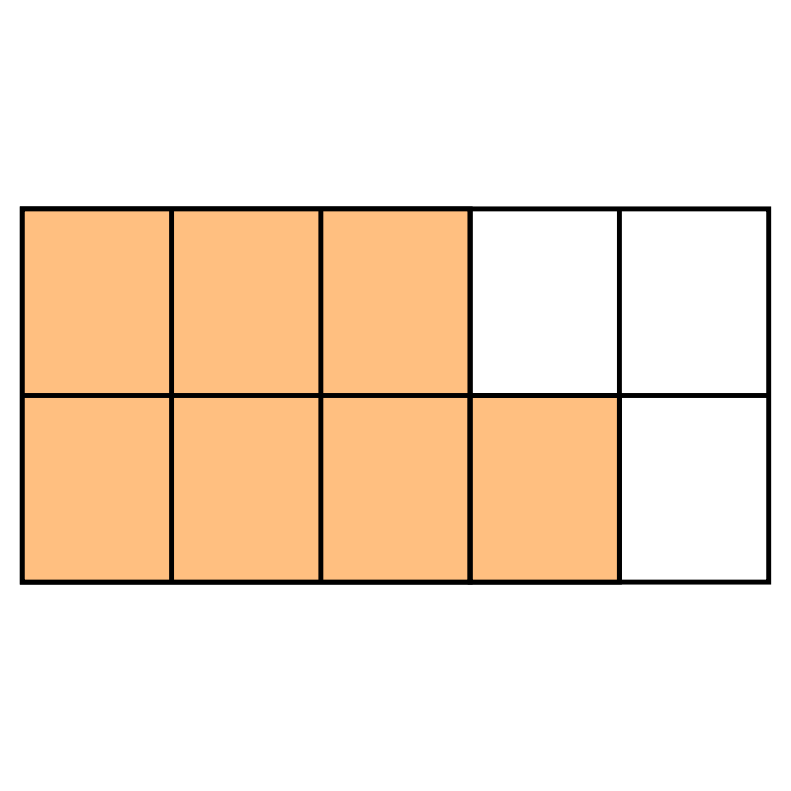
\includegraphics[width=65px]{../images/imagen_frac_5prim_7|10.png} \fillin[\fbox{$\dfrac{7}{10}$}][0in] \\[-0.5em]
				\part 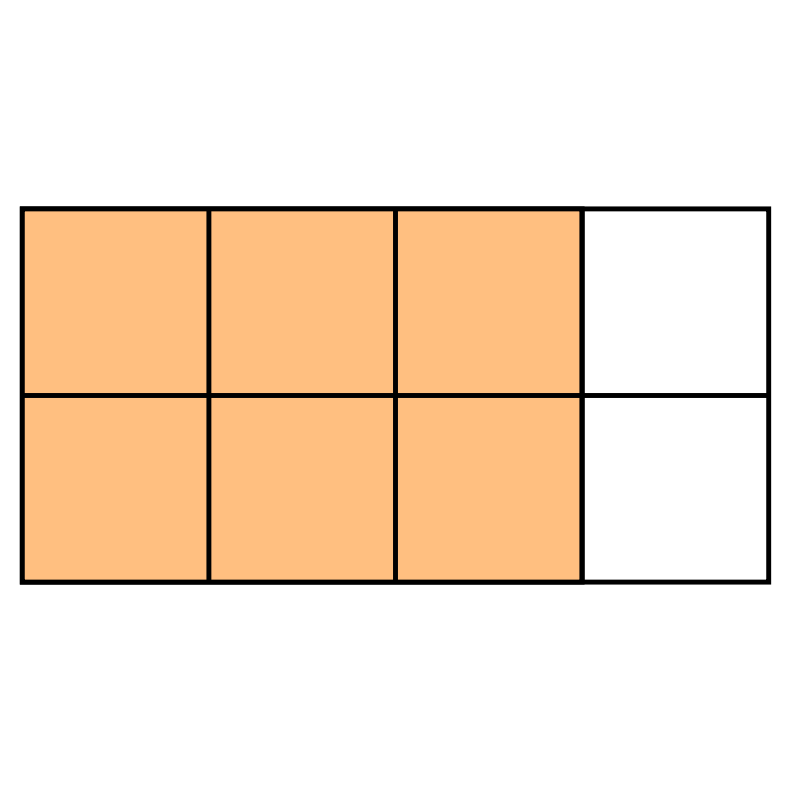
\includegraphics[width=65px]{../images/imagen_frac_5prim_6|8.png} \fillin[\fbox{$\dfrac{6}{8}$}][0in] \\[-0.5em]
				% \part 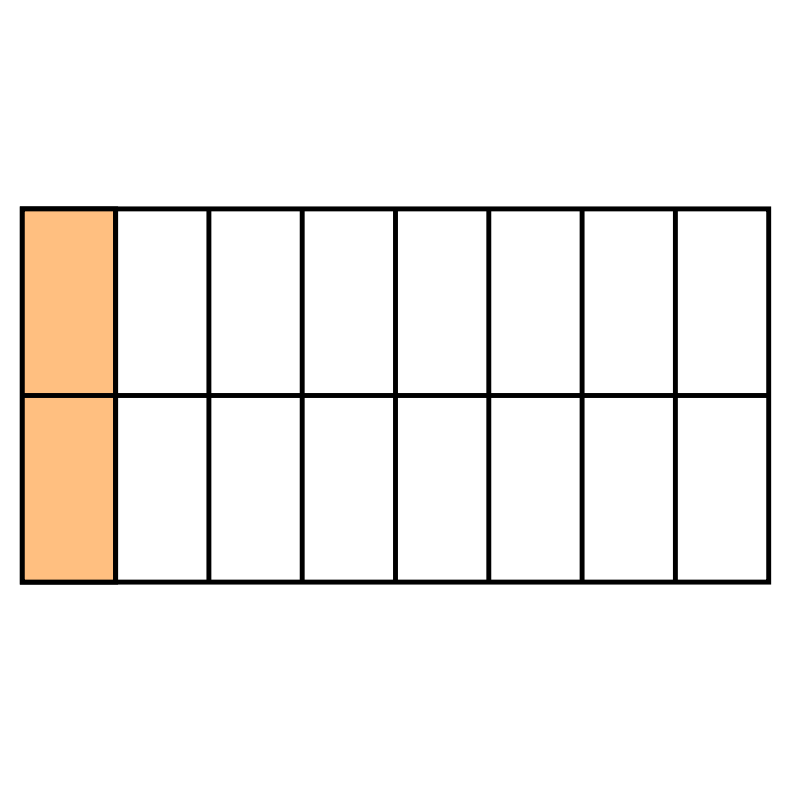
\includegraphics[width=50px]{../images/imagen_frac_5prim_2|16.png} \fillin[\fbox{$\dfrac{2}{16}$}][0in] \\[-0.5em]
				% \part 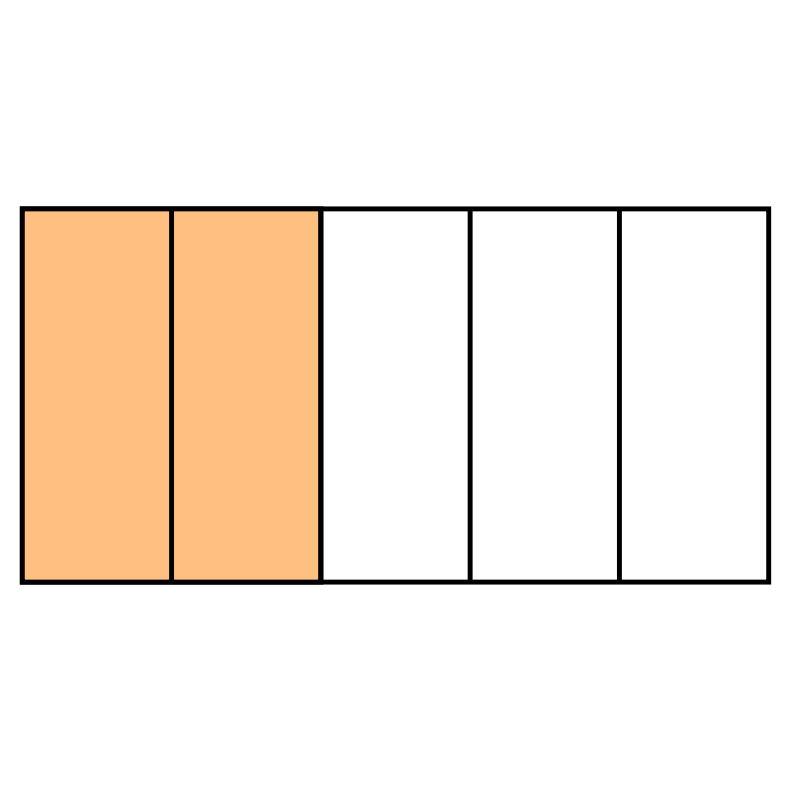
\includegraphics[width=50px]{../images/imagen_frac_5prim_2|5.png} \fillin[\fbox{$\dfrac{2}{5}$}][0in] \\[-0.5em]
				% \part 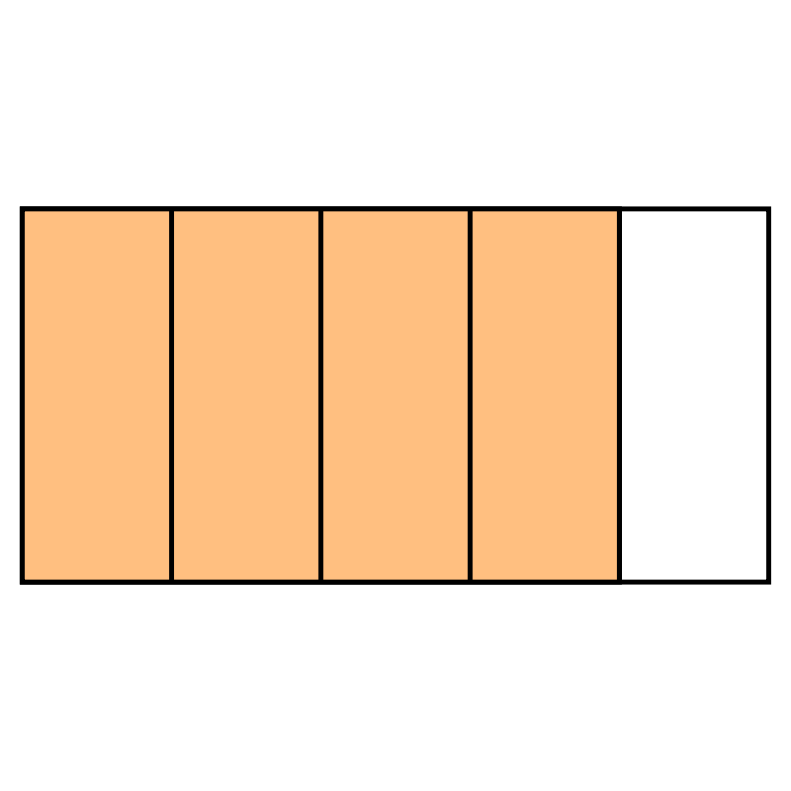
\includegraphics[width=50px]{../images/imagen_frac_5prim_4|5.png} \fillin[\fbox{$\dfrac{4}{5}$}][0in] \\[-0.5em]
				% \part 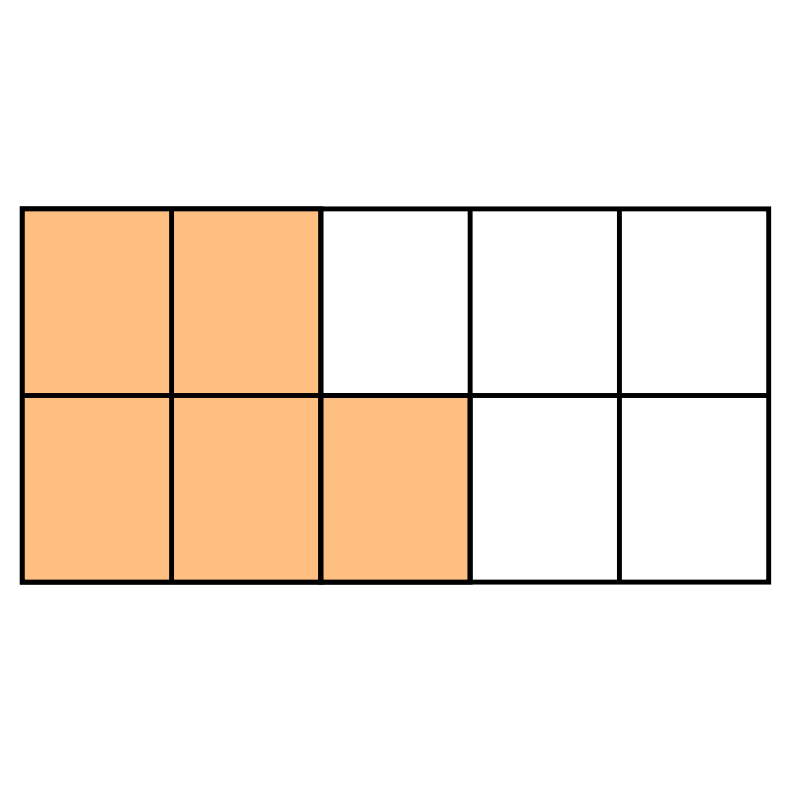
\includegraphics[width=50px]{../images/imagen_frac_5prim_5|10.png} \fillin[\fbox{$\dfrac{5}{10}$}][0in] \\[-0.5em]
				% \part 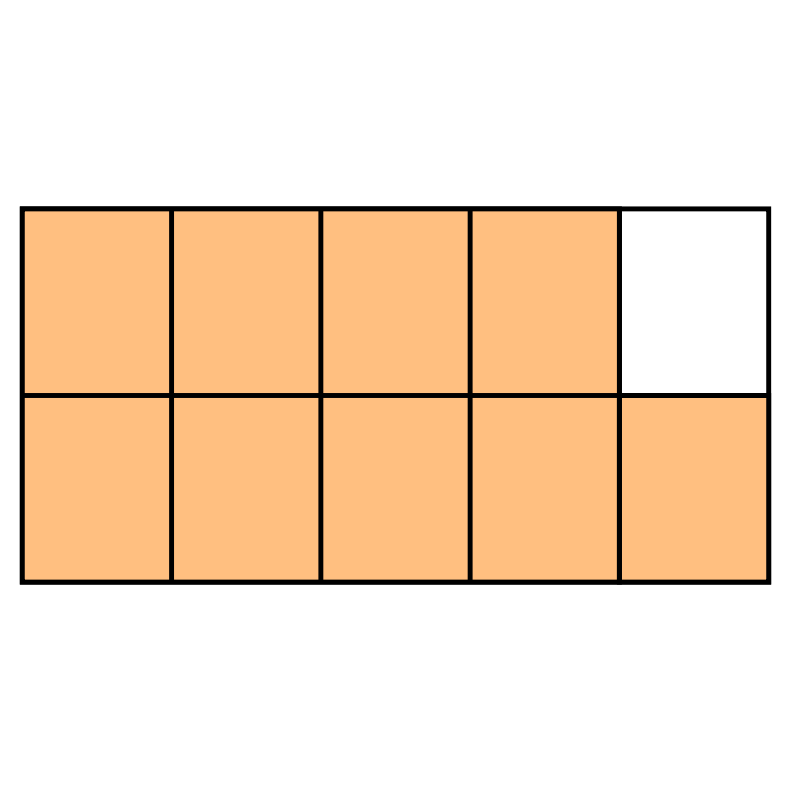
\includegraphics[width=50px]{../images/imagen_frac_5prim_9|10.png} \fillin[\fbox{$\dfrac{9}{10}$}][0in] \\[-0.5em]
				% \part 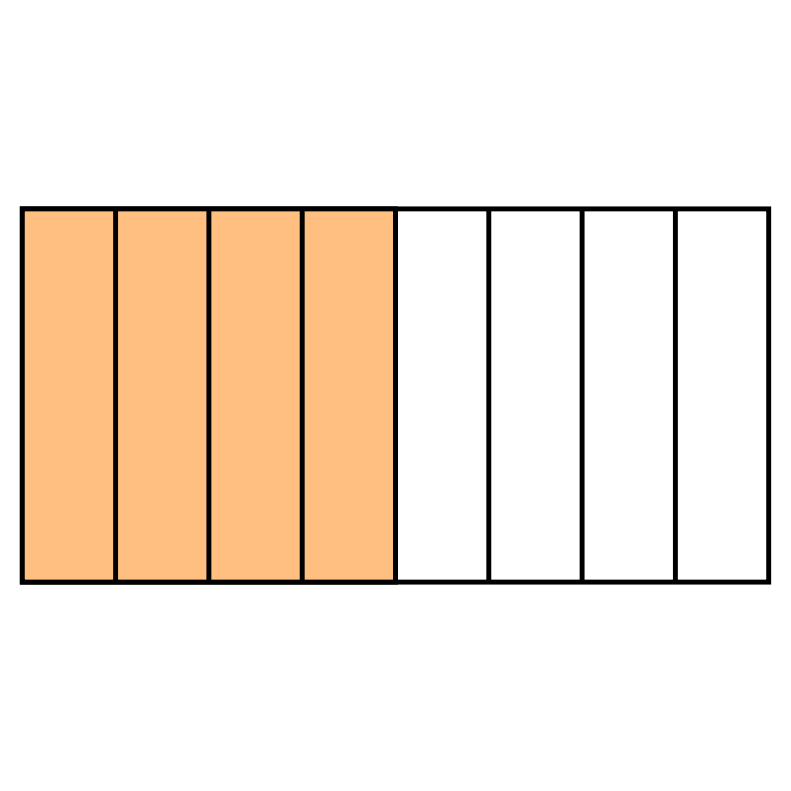
\includegraphics[width=50px]{../images/imagen_frac_5prim_4|8.png} \fillin[\fbox{$\dfrac{4}{8}$}][0in] \\[-0.5em]
				% \part 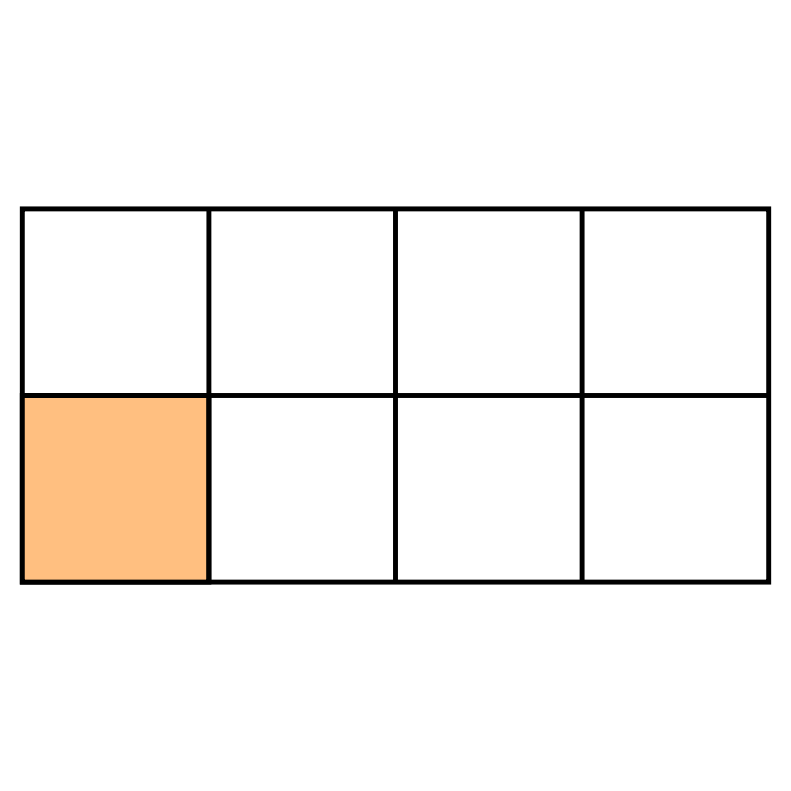
\includegraphics[width=50px]{../images/imagen_frac_5prim_1|8.png} \fillin[\fbox{$\dfrac{1}{8}$}][0in] \\[-0.5em]
				% \part 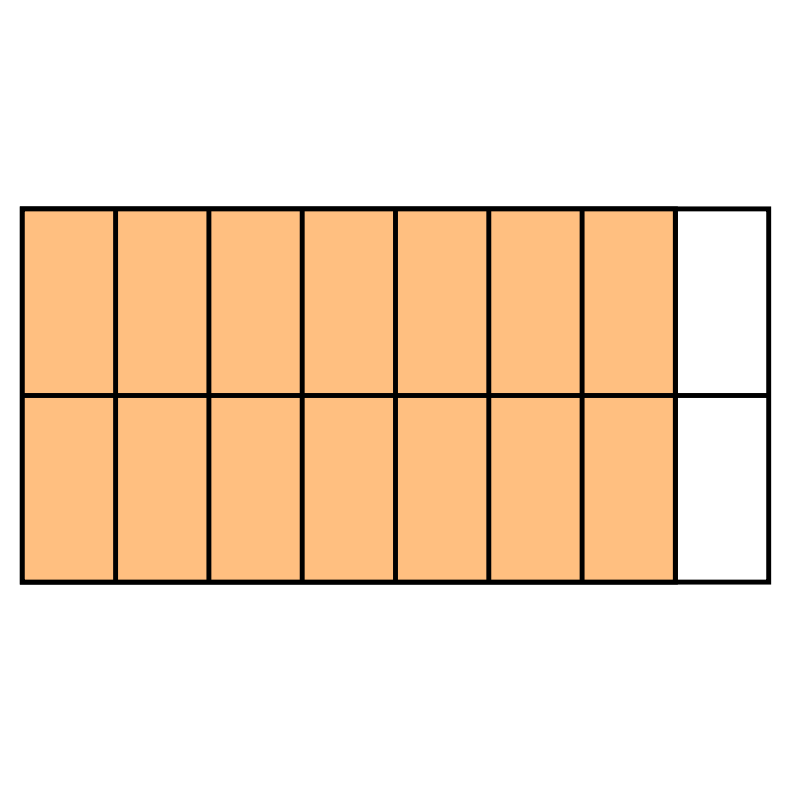
\includegraphics[width=50px]{../images/imagen_frac_5prim_14|16.png} \fillin[\fbox{$\dfrac{14}{16}$}][0in] \\[-0.5em]
				% \part 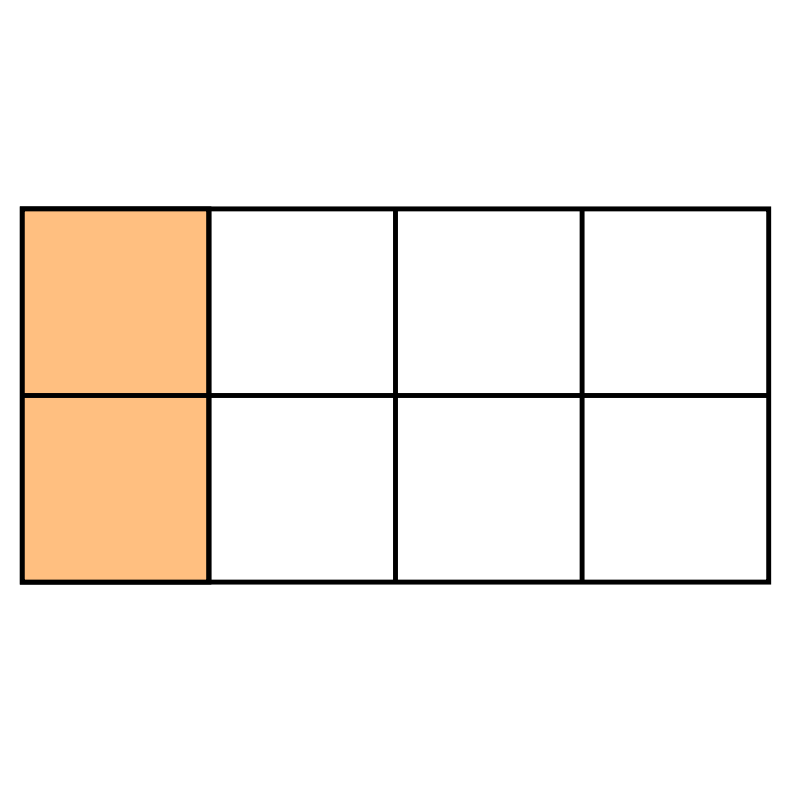
\includegraphics[width=50px]{../images/imagen_frac_5prim_2|8.png} \fillin[\fbox{$\dfrac{2}{8}$}][0in] \\[-0.5em]
				\part 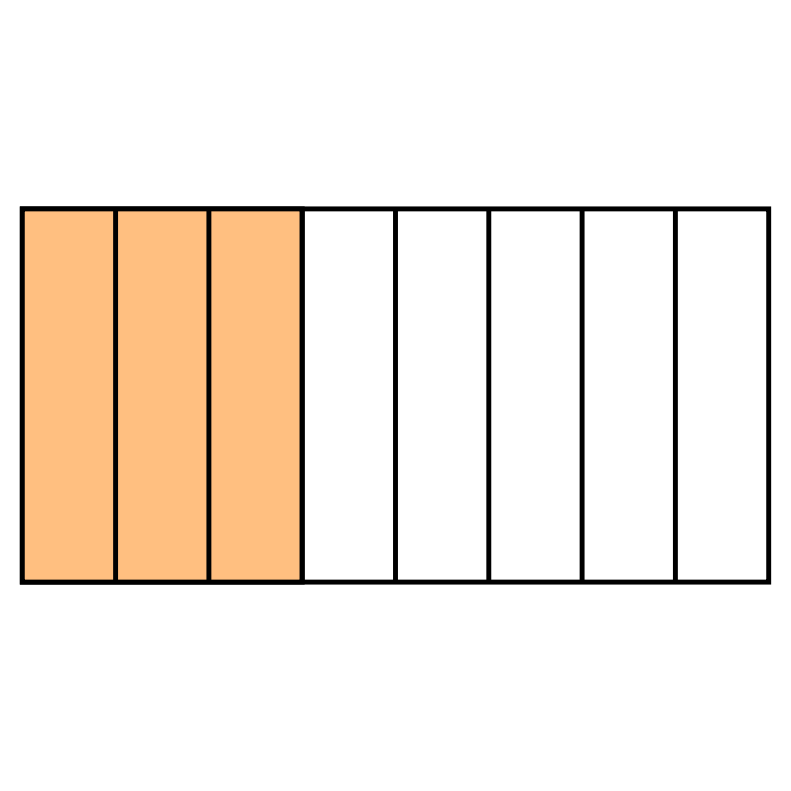
\includegraphics[width=65px]{../images/imagen_frac_5prim_3|8.png} \fillin[\fbox{$\dfrac{3}{8}$}][0in] \\[-0.5em]
				% \part 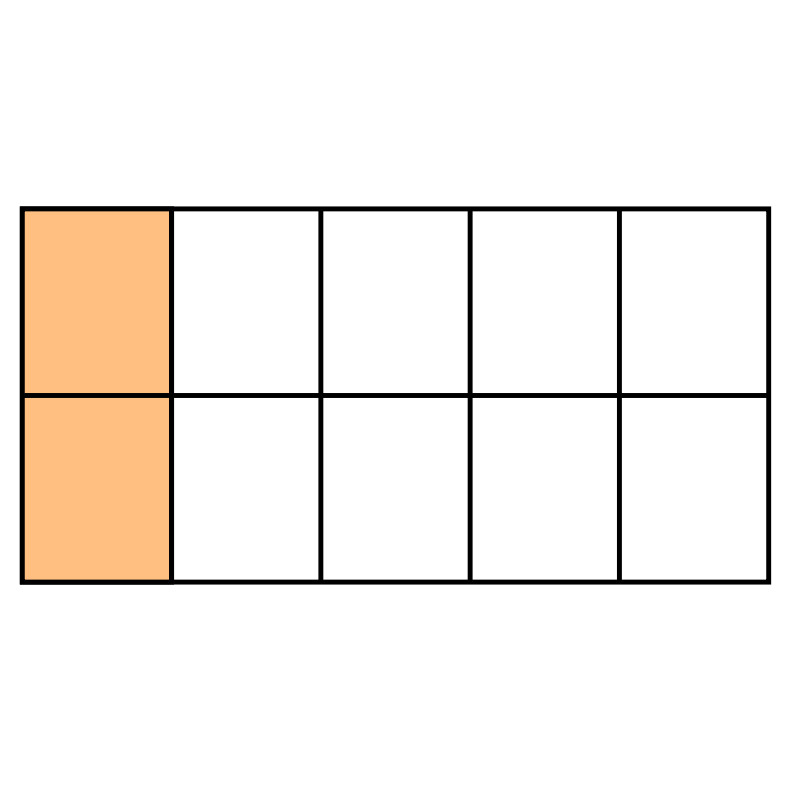
\includegraphics[width=50px]{../images/imagen_frac_5prim_2|10.png} \fillin[\fbox{$\dfrac{2}{10}$}][0in] \\[-0.5em]
				% \part 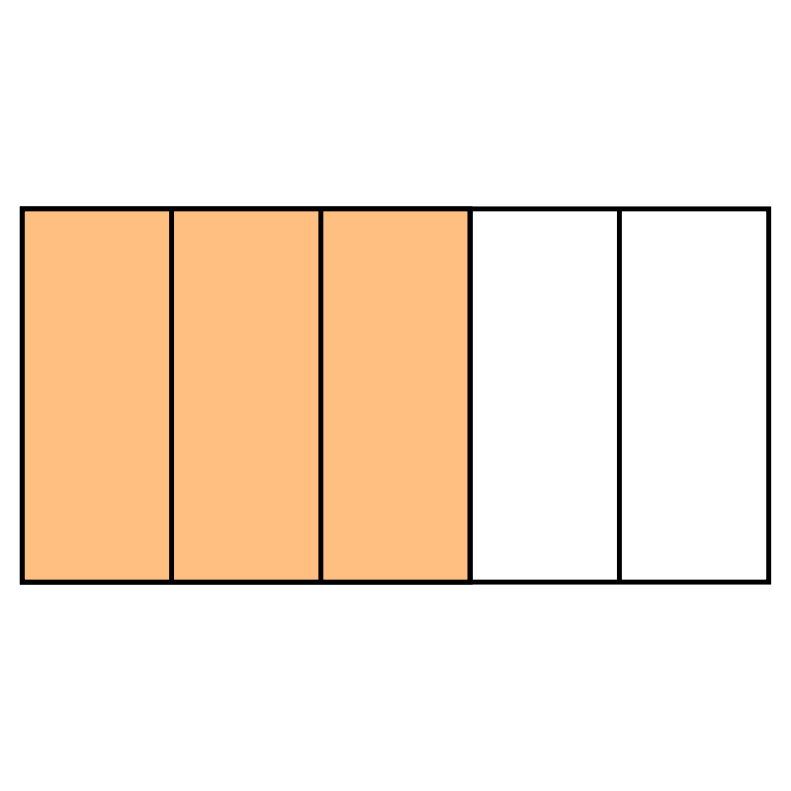
\includegraphics[width=50px]{../images/imagen_frac_5prim_3|5.png} \fillin[\fbox{$\dfrac{3}{5}$}][0in] \\[-0.5em]
				\part 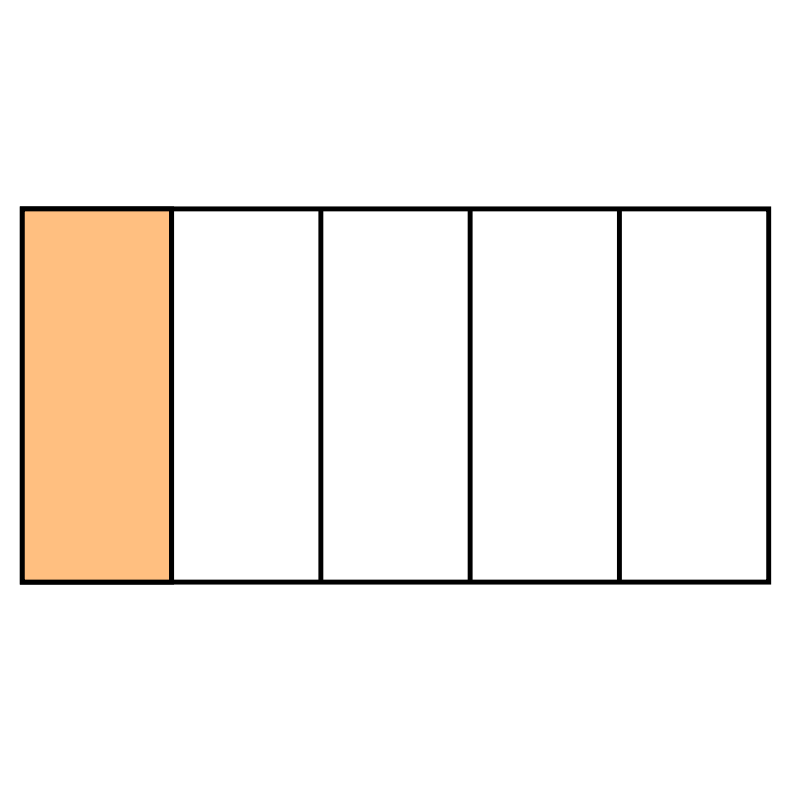
\includegraphics[width=65px]{../images/imagen_frac_5prim_1|5.png} \fillin[\fbox{$\dfrac{1}{5}$}][0in] \\[-0.5em]
				% \part 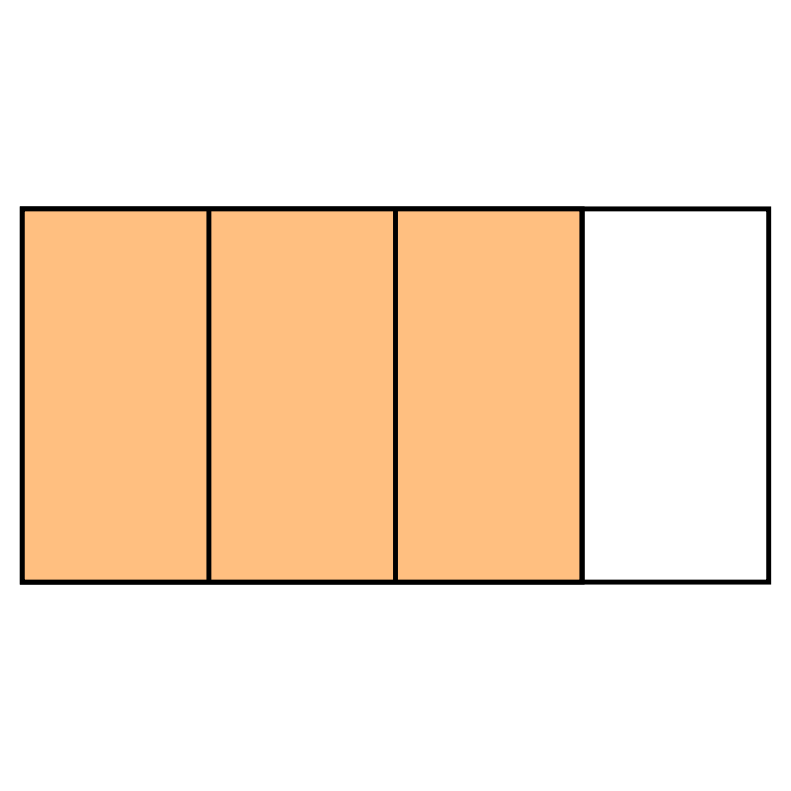
\includegraphics[width=50px]{../images/imagen_frac_5prim_3|4.png} \fillin[\fbox{$\dfrac{3}{4}$}][0in] \\[-0.5em]
			\end{parts}
		\end{multicols}
	}

	% \addcontentsline{toc}{subsubsection}{Nombre de fracciones}
	% \subsubsection*{Nombre de fracciones}

	\question[2]{Escribe la fracción que corresponda en cada inciso:

		\begin{parts}
			\part ¿Cómo se escribe numéricamente la fracción \textbf{siete catorceavos}?    \fillin[$\dfrac{7}{14}$][0in]
			% \part ¿Cómo se escribe numéricamente la fracción \textbf{ocho onceavos}?   \fillin[$\dfrac{8}{11}$][0in]
			% \part ¿Cómo se escribe numéricamente la fracción \textbf{doce séptimos}?    \fillin[$\dfrac{12}{7}$][0in]
			\part ¿Cómo se escribe numéricamente la fracción \textbf{nueve treceavos}?     \fillin[$\dfrac{9}{13}$][0in]
		\end{parts}
	}

	% \addcontentsline{toc}{subsubsection}{Fracciones en la recta numérica}
	% \subsubsection*{Fracciones en la recta numérica}
	\question[2]{Escribe la fracción que representa el punto en la recta numérica de cada imagen:

		\begin{multicols}{2}
			\begin{parts}
				\part 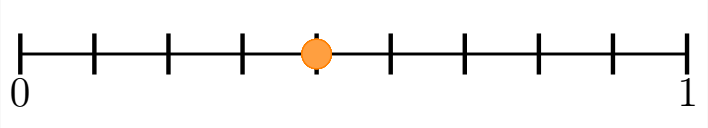
\includegraphics[width=180px]{../images/recta_num_frac4|9.png}   \hfill \fillin[\fbox{$\dfrac{ 4}{9 }$}][0in]
				% \part 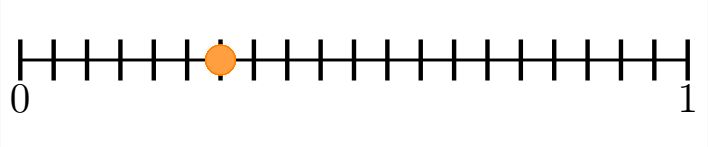
\includegraphics[width=180px]{../images/recta_num_frac6|20.png}  \hfill \fillin[\fbox{$\dfrac{ 6}{20}$}][0in]
				\part 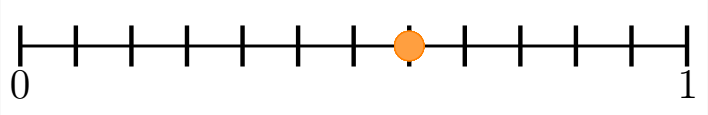
\includegraphics[width=180px]{../images/recta_num_frac7|12.png}  \hfill \fillin[\fbox{$\dfrac{ 7}{12}$}][0in]
				% \part 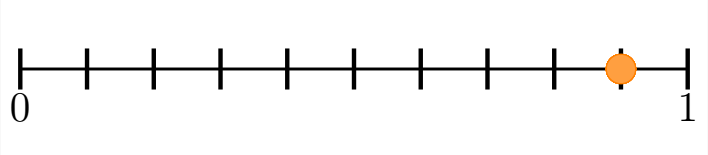
\includegraphics[width=180px]{../images/recta_num_frac9|10.png}  \hfill \fillin[\fbox{$\dfrac{ 9}{10}$}][0in]
				% \part 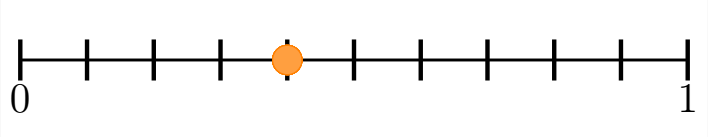
\includegraphics[width=180px]{../images/recta_num_frac4|10.png}  \hfill \fillin[\fbox{$\dfrac{ 4}{10}$}][0in]
				% \part 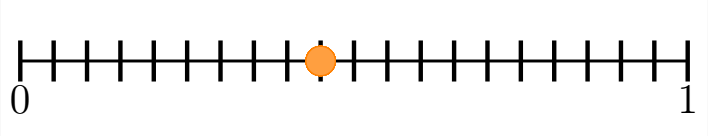
\includegraphics[width=180px]{../images/recta_num_frac9|20.png}  \hfill \fillin[\fbox{$\dfrac{ 9}{20}$}][0in]
				\part 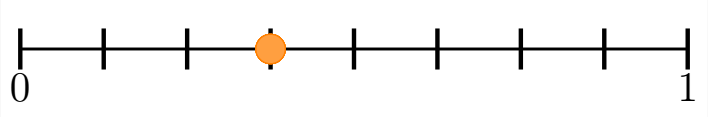
\includegraphics[width=180px]{../images/recta_num_frac3|8.png}   \hfill \fillin[\fbox{$\dfrac{ 3}{8 }$}][0in]
				% \part 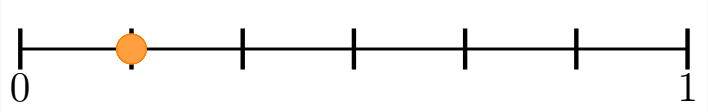
\includegraphics[width=180px]{../images/recta_num_frac1|6.png}   \hfill \fillin[\fbox{$\dfrac{ 1}{6 }$}][0in]
				\part 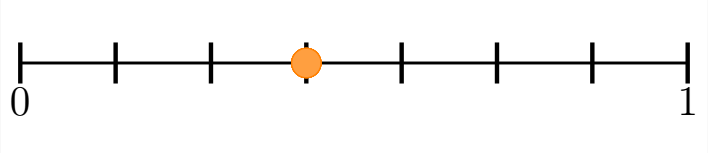
\includegraphics[width=180px]{../images/recta_num_frac3|7.png}   \hfill \fillin[\fbox{$\dfrac{ 3}{7 }$}][0in]
				% \part 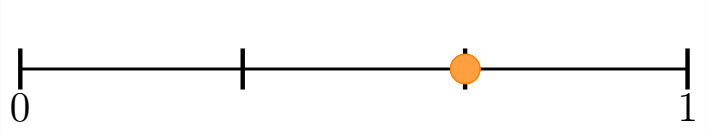
\includegraphics[width=180px]{../images/recta_num_frac2|3.png}   \hfill \fillin[\fbox{$\dfrac{ 2}{3 }$}][0in]
			\end{parts}
		\end{multicols}
	}

	% \addcontentsline{toc}{subsubsection}{Conversión de fracciones}
	% \subsubsection*{Conversión de fracciones}

	\question[2]{Convierte la siguientes fracciones mixtas a impropias y viseversa:

		\begin{multicols}{3}
			\begin{parts}
				\part $4\dfrac{2}{3}= $  \fillin[$\dfrac{14}{3}$][0in]\\
				\part $\dfrac{13}{3}= $  \fillin[$4\dfrac{1}{3}$][0in]\\
				% \part $2\dfrac{3}{10}= $ \fillin[$\dfrac{23}{10}$][0in]\\
				% \part $\dfrac{43}{10}= $ \fillin[$4\dfrac{3}{10}$][0in]\\
				% \part $5\dfrac{1}{5}= $  \fillin[$\dfrac{26}{5}$][0in]\\
				% \part $\dfrac{51}{5}= $  \fillin[$10\dfrac{1}{5}$][0in]\\
			\end{parts}
		\end{multicols}
	}

	\addcontentsline{toc}{subsection}{Simplificación de fracciones}
	\subsection*{Simplificación de fracciones}
	% \addcontentsline{toc}{subsubsection}{Comparación de fracciones}
	% \subsubsection*{Comparación de fracciones}

	\question[2]{Escribe sobre la línea el símbolo de mayor que ($>$), menor que ($<$), o igual ($=$) según corresponda.

		\begin{multicols}{5}
			\begin{parts}
				% \part $\dfrac{2}{5}$ \fillin[$>$][0.5in] $\dfrac{1}{3}$\\[0.25em]
				\part $\dfrac{3}{4}$ \fillin[$>$][0.5in] $\dfrac{3}{5}$\\[0.25em]
				\part $\dfrac{2}{5}$ \fillin[$<$][0.5in] $\dfrac{2}{3}$\\[0.25em]
				\part $\dfrac{3}{2}$ \fillin[$=$][0.5in] $\dfrac{9}{6}$\\[0.25em]
				% \part $\dfrac{5}{6}$ \fillin[$>$][0.5in] $\dfrac{4}{6}$\\[0.25em]
				% \part $\dfrac{4}{3}$ \fillin[$>$][0.5in] $\dfrac{5}{4}$\\[0.25em]
				\part $\dfrac{1}{3}$ \fillin[$>$][0.5in] $\dfrac{9}{3}$\\[0.25em]
				% \part $\dfrac{2}{3}$ \fillin[$<$][0.5in] $\dfrac{3}{2}$\\[0.25em]
				\part $\dfrac{1}{4}$ \fillin[$<$][0.5in] $\dfrac{2}{3}$\\[0.25em]
				% \part $\dfrac{5}{6}$ \fillin[$>$][0.5in] $\dfrac{4}{5}$\\[0.25em]
			\end{parts}
		\end{multicols}
	}


	% \addcontentsline{toc}{subsubsection}{Mínimo común múltiplo}
	% \subsubsection*{Mínimo común múltiplo}
	% \addcontentsline{toc}{subsubsection}{Máximo común divisor}
	% \subsubsection*{Máximo común divisor}
\newpage
	\question[4]{Calcula lo que se te pide en cada inciso:

		% \begin{multicols}{2}
		\begin{parts}
			% \part Encuentra el mínimo común múltiplo de 2 y 9.     	\hfill\fillin[El MCM de 2 y 9 es 18.][0in] \\[0.8em]
			% \part Encuentra el máximo común divisor de 5 y 15.     	\hfill\fillin[El MCD de 5 y 15 es 5.][0in] \\[0.8em]
			% \part Encuentra el máximo común divisor de 33 y 121.   	\hfill\fillin[El MCD de 33 y 121 es 11.][0in] \\[0.8em]
			\part El máximo común divisor de 15 y 100.   	\hfill \fillin[El MCD de 25 y 100 es 25.][0in] 
			% \part Encuentra el máximo común divisor de 18 y 36.    	\hfill\fillin[El MCD de 18 y 36 es 18.][0in] \\[0.8em]
			% \part Encuentra el mínimo común múltiplo de 4 y 9.     	\hfill\fillin[El MCM de 4 y 9 es 36.][0in] \\[0.8em]
			% \part Encuentra el mínimo común múltiplo de 6 y 7.     	\hfill\fillin[El MCM de 6 y 7 es 42.][0in] \\[0.8em]
			% \part Encuentra el mínimo común múltiplo de 2, 3 y 4.  	\hfill\fillin[El MCM de 2, 3 y 4 es 12.][0in] \\[0.8em]
			% \part Encuentra el máximo común divisor de 2 y 14.     	\hfill\fillin[El MCD de 2 y 14 es 2.][0in] \\[0.8em]
			\part El mínimo común múltiplo de 12 y 18. \hfill \fillin[El MCM de 12 y 18 es 36.][0in]
		\end{parts}
		% \end{multicols}
	}
	% \addcontentsline{toc}{subsubsection}{Simplificación de fracciones}
	% \subsubsection*{Simplificación de fracciones}

	\question[2]{Simplifica a su mínima expresión las siguientes fracciones usando el máximo común divisor:

		\begin{multicols}{5}
			\begin{parts}
				% \part $\dfrac{12}{48}= $  \fillin[$\dfrac{1}{4}$][0in]\\[0.5em]
				\part $\dfrac{6}{24}= $  \fillin[$\dfrac{1}{4}$][0in]
				\part $\dfrac{16}{36}= $  \fillin[$\dfrac{4}{9}$][0in]
				% \part $\dfrac{4}{40}= $  \fillin[$\dfrac{1}{10}$][0in]\\[0.5em]
				% \part $\dfrac{4}{20}= $  \fillin[$\dfrac{1}{5}$][0in]\\[0.5em]
				% \part $\dfrac{2}{30}= $  \fillin[$\dfrac{1}{15}$][0in]\\[0.5em]
				% \part $\dfrac{6}{36}= $  \fillin[$\dfrac{1}{6}$][0in]\\[0.5em]
				% \part $\dfrac{5}{25}= $  \fillin[$\dfrac{1}{5}$][0in]\\[0.5em]
				\part $\dfrac{6}{30}= $  \fillin[$\dfrac{1}{5}$][0in]
				% \part $\dfrac{2}{12}= $  \fillin[$\dfrac{1}{6}$][0in]\\[0.5em]
				% \part $\dfrac{4}{16}= $  \fillin[$\dfrac{1}{4}$][0in]\\[0.5em]
				\part $\dfrac{15}{20}= $  \fillin[$\dfrac{3}{4}$][0in]
				% \part $\dfrac{5}{50}= $  \fillin[$\dfrac{1}{10}$][0in]\\[0.5em]
				% \part $\dfrac{6}{10}= $  \fillin[$\dfrac{3}{5}$][0in]\\[0.5em]
				\part $\dfrac{3}{18}= $  \fillin[$\dfrac{1}{6}$][0in]
			\end{parts}
		\end{multicols}
	}
	
	% \addcontentsline{toc}{subsubsection}{Fracciones equivalentes}
	% \subsubsection*{Fracciones equivalentes}

	\question[2]{Indica si las siguientes fracciones son equivalentes o no:

		\begin{multicols}{2}
			\begin{parts}

				\part $\dfrac{1}{2}=\dfrac{4}{6}$\qquad
				\begin{oneparcheckboxes}
					\choice Sí
					\CorrectChoice No
				\end{oneparcheckboxes}

				\part $\dfrac{4}{5}=\dfrac{8}{10}$\qquad
				\begin{oneparcheckboxes}
					\CorrectChoice Sí
					\choice No
				\end{oneparcheckboxes}

				\part $\dfrac{1}{8}=\dfrac{4}{16}$\qquad
				\begin{oneparcheckboxes}
					\choice Sí
					\CorrectChoice No
				\end{oneparcheckboxes}

				\part $\dfrac{1}{5}=\dfrac{5}{10}$\qquad
				\begin{oneparcheckboxes}
					\choice Sí
					\CorrectChoice No
				\end{oneparcheckboxes}

				% \part $\dfrac{1}{10}=\dfrac{3}{30}$\qquad
				% \begin{oneparcheckboxes}
				% 	\CorrectChoice Sí
				% 	\choice No
				% \end{oneparcheckboxes}

				% \part $\dfrac{1}{4}=\dfrac{2}{4}$\qquad
				% \begin{oneparcheckboxes}
				% 	\choice Sí
				% 	\CorrectChoice No
				% \end{oneparcheckboxes}

				% \part $\dfrac{1}{5}=\dfrac{10}{25}$\qquad
				% \begin{oneparcheckboxes}
				% 	\choice Sí
				% 	\CorrectChoice No
				% \end{oneparcheckboxes}

				% \part $\dfrac{3}{2}=\dfrac{12}{8}$\qquad
				% \begin{oneparcheckboxes}
				% 	\CorrectChoice Sí
				% 	\choice No
				% \end{oneparcheckboxes}

				% \part $\dfrac{3}{6}=\dfrac{1}{3}$\qquad
				% \begin{oneparcheckboxes}
				% 	\choice Sí
				% 	\CorrectChoice No
				% \end{oneparcheckboxes}

				% \part $\dfrac{18}{12}=\dfrac{9}{4}$\qquad
				% \begin{oneparcheckboxes}
				% 	\choice Sí
				% 	\CorrectChoice No
				% \end{oneparcheckboxes}
			\end{parts}
		\end{multicols}
	}


	

	\addcontentsline{toc}{subsection}{Suma, resta, multiplicación y división de fracciones}
	\subsection*{Suma, resta, multiplicación y división de fracciones}
	% \addcontentsline{toc}{subsubsection}{Simplificación de fracciones}
	% \subsubsection*{Simplificación de fracciones}
	% \addcontentsline{toc}{subsubsection}{Suma y resta con denominadores iguales}
	% \subsubsection*{Suma y resta con denominadores iguales}
	% \addcontentsline{toc}{subsubsection}{Suma y resta denominadores diferentes 1}
	% \subsubsection*{Suma y resta denominadores diferentes 1}
	% \addcontentsline{toc}{subsubsection}{Suma y resta denominadores diferentes 2}
	% \subsubsection*{Suma y resta denominadores diferentes 2}

	\question[2]{Realiza las siguientes operaciones con fracciones (Expresa tu resultado como una \textbf{fracción mixta simplificada}), según sea el caso:

		\begin{multicols}{3}
			\begin{parts}
				% \part $\dfrac{3}{5}+\dfrac{4}{5}=$ \fillin[$\dfrac{7}{5} = 1\dfrac{2}{5}$][0in] \\[1em]
				\part $\dfrac{3}{10}+\dfrac{4}{5}=$ \fillin[$\dfrac{11}{10} = 1\dfrac{1}{10}$][0in] \\[0.2em]
				\part $\dfrac{2}{7}\divisionsymbol\dfrac{2}{5}=$ \fillin[$\dfrac{5}{7}$][0in]   \\[0.2em]
				\part $\dfrac{13}{6}-\dfrac{5}{6}=$ \fillin[$\dfrac{8}{6}=\dfrac{4}{3}$][0in] \\[0.2em]
				% \part $\dfrac{9}{10}+\dfrac{2}{3}=$ \fillin[$1\dfrac{17}{30}$][0in] \\[1em]
				\part $3\times\dfrac{5}{4}=$ \fillin[$\dfrac{15}{4}$][0in]   \\[0.2em]
				% \part $1\dfrac{1}{2}+1\dfrac{2}{3}=$ \fillin[$3\dfrac{1}{6}$][0in] \\[1em]
				\part $3\dfrac{3}{4}-2\dfrac{2}{3}=$ \fillin[$1\dfrac{1}{12}$][0in] \\[0.2em]
				\part $4\divisionsymbol\dfrac{3}{5}=$ \fillin[$\dfrac{20}{3}$][0in]   \\[0.2em]
				% \part $2\dfrac{2}{3}\divisionsymbol 1\dfrac{3}{4}=$ \fillin[$\dfrac{32}{21}$][0in]   \\[1em]
			\end{parts}
		\end{multicols}
	}

	%%% \addcontentsline{toc}{subsubsection}{Resolución de problemas}
	%%% \subsubsection*{Resolución de problemas}

	% \addcontentsline{toc}{subsection}{Multiplicación y división de fracciones}
	% \subsection*{}
	% \addcontentsline{toc}{subsubsection}{Multiplicación de fracciones}
	% \subsubsection*{Multiplicación de fracciones}
	% \addcontentsline{toc}{subsubsection}{División de fracciones}
	% \subsubsection*{División de fracciones}
	% \addcontentsline{toc}{subsubsection}{Multiplicación y división 1}
	% \subsubsection*{Multiplicación y división 1}
	% \addcontentsline{toc}{subsubsection}{Multiplicación y división 2}
	% \subsubsection*{Multiplicación y división 2}


	% \question[2]{Realiza las siguientes operaciones de multiplicación y división de fracciones (Expresa tu resultadocomo una \textbf{fracción simplificada}):

	% 	\begin{multicols}{4}
	% 		\begin{parts}
	% 			\part $\dfrac{7}{9}\times\dfrac{12}{17}=$ \fillin[$\dfrac{28}{51}$][0in]   \\[1em]
	% 			\part $\dfrac{2}{7}\divisionsymbol\dfrac{2}{5}=$ \fillin[$\dfrac{5}{7}$][0in]   \\[1em]
	% 			\part $3\times\dfrac{5}{4}=$ \fillin[$\dfrac{15}{4}$][0in]   \\[1em]
	% 			\part $1\dfrac{1}{4}\times 4\dfrac{5}{8}=$ \fillin[$\dfrac{185}{32}$][0in]   \\[1em]
	% 			\part $\dfrac{5}{6}\times\dfrac{4}{5}=$ \fillin[$\dfrac{2}{3}$][0in]   \\[1em]
	% 			\part $\dfrac{4}{7}\divisionsymbol\dfrac{5}{6}=$ \fillin[$\dfrac{24}{35}$][0in]   \\[1em]
	% 			\part $\dfrac{7}{6}\times 6=$ \fillin[$\dfrac{21}{2}$][0in]   \\[1em]
	% 			\part $3\dfrac{1}{3}\times 2\dfrac{2}{5}=$ \fillin[$8$][0in]   \\[1em]
	% 			\part $\dfrac{3}{7}\times\dfrac{5}{6}=$ \fillin[$\dfrac{5}{14}$][0in]   \\[1em]
	% 			\part $\dfrac{7}{8}\divisionsymbol\dfrac{5}{4}=$ \fillin[$\dfrac{7}{10}$][0in]   \\[1em]
	% 			\part $\dfrac{2}{5}\divisionsymbol 5=$ \fillin[$\dfrac{2}{25}$][0in]   \\[1em]
	% 			\part $6\dfrac{1}{2}\divisionsymbol 1\dfrac{5}{7}=$ \fillin[$\dfrac{91}{24}$][0in]   \\[1em]
	% 			\part $\dfrac{5}{8}\times\dfrac{4}{5}=$ \fillin[$\dfrac{1}{2}$][0in]   \\[1em]
	% 			\part $\dfrac{6}{7}\divisionsymbol\dfrac{1}{3}=$ \fillin[$\dfrac{18}{7}$][0in]   \\[1em]
	% 			\part $4\divisionsymbol\dfrac{3}{5}=$ \fillin[$\dfrac{20}{3}$][0in]   \\[1em]
	% 			\part $2\dfrac{2}{3}\divisionsymbol 1\dfrac{3}{4}=$ \fillin[$\dfrac{32}{21}$][0in]   \\[1em]
	% 		\end{parts}
	% 	\end{multicols}
	% }

	%%% \addcontentsline{toc}{subsubsection}{Resolución de problemas}
	%%% \subsubsection*{Resolución de problemas}

	\addcontentsline{toc}{subsection}{Porcentajes}
	\subsection*{Porcentajes}
	% \addcontentsline{toc}{subsubsection}{Porcentajes a decimales}
	% \subsubsection*{Porcentajes a decimales}

	\question[2]{Escribe los siguientes porcentajes como números decimales:

		\begin{multicols}{4}
			\begin{parts}
				% \part $14\%=$ \fillin[\fbox{0.14}][0cm] \\
				% \part $73\%=$ \fillin[\fbox{0.73}][0cm] \\
				% \part $15\%=$ \fillin[\fbox{0.15}][0cm] \\
				% \part $85\%=$ \fillin[\fbox{0.85}][0cm] \\
				\part $91\%=$ \fillin[\fbox{0.91}][0cm] \\
				\part $19\%=$ \fillin[\fbox{0.19}][0cm] \\
				% \part $ 9\%=$ \fillin[\fbox{0.09}][0cm] \\
				\part $42\%=$ \fillin[\fbox{0.42}][0cm] \\
				% \part $25\%=$ \fillin[\fbox{0.25}][0cm] \\
				% \part $ 3\%=$ \fillin[\fbox{0.03}][0cm] \\
				% \part $ 8\%=$ \fillin[\fbox{0.08}][0cm] \\
				\part $ 2\%=$ \fillin[\fbox{0.02}][0cm] \\
			\end{parts}
		\end{multicols}
	}

	% \addcontentsline{toc}{subsubsection}{Decimales a porcentajes}
	% \subsubsection*{Decimales a porcentajes}

	\question[2]{Escribe el porcentaje que representa cada número decimal:

		\begin{multicols}{3}
			\begin{parts}
				\part $0.248=$ \fillin[\fbox{$24.8\%$}][0cm]
				% \part $0.46=$  \fillin[\fbox{$\dfrac{23}{50}$}][0cm]
				% \part $0.24=$  \fillin[\fbox{$\dfrac{6}{25}$}][0cm]
				% \part $0.9=$   \fillin[\fbox{$\dfrac{9}{10}$}][0cm]
				% \part $0.115=$ \fillin[\fbox{$\dfrac{23}{200}$}][0cm]
				% \part $0.66=$  \fillin[\fbox{$\dfrac{33}{50}$}][0cm]
				\part $0.06=$  \fillin[\fbox{$6\&$}][0cm]
				% \part $0.58=$  \fillin[\fbox{$\dfrac{29}{50}$}][0cm]
			\end{parts}
		\end{multicols}
	}

	%%% \addcontentsline{toc}{subsubsection}{50\%, 25\%, 10\% y 1\%}
	%%% \subsubsection*{50\%, 25\%, 10\% y 1\%}


	% \addcontentsline{toc}{subsubsection}{Porcentajes de cantidades}
	% \subsubsection*{Porcentajes de cantidades}

	\question[3]{Calcula los porentajes de los siguientes números:

	\begin{multicols}{3}
		\begin{parts}
			% \part ¿Cuál es el 80\% de 660?   \hfill \fillin[\fbox{528}][0cm]
			\part ¿Cuál es el 20\% de 50?    \hfill \fillin[\fbox{10}][0cm]
			% \part ¿Cuál es el 50\% de 862?   \hfill \fillin[\fbox{431}][0cm]
			\part ¿Cuál es el 30\% de 300?   \hfill \fillin[\fbox{90}][0cm]
			% \part ¿Cuál es el 20\% de 415?   \hfill \fillin[\fbox{83}][0cm]
			% \part ¿Cuál es el 12\% de 338?   \hfill \fillin[\fbox{40.56}][0cm]
			\part ¿Cuál es el 14\% de 710?   \hfill \fillin[\fbox{99.4}][0cm]
			% \part ¿Cuál es el 80\% de 1260?  \hfill \fillin[\fbox{1008}][0cm]
		\end{parts}
	\end{multicols}
}

	% \addcontentsline{toc}{subsubsection}{Resolución de problemas}
	% \subsubsection*{Resolución de problemas}

	\question[2]{Resuelve los siguientes problemas:

	\begin{multicols}{2}
		\begin{parts}
			\part El costo de una camisa es de \$800 pesos, si se les hace un descuento del 20\%, ¿cuánto pagaré en total por la camisa?

			\begin{solutionbox}{1.8cm}
				\[\$800\times 20\%=\$160\]
				\[\$800-\$160=\$640\]
			\end{solutionbox}

			% \part El 24\% de los habitantes de un pueblo tienen menos de 30 años. ¿Cuántos habitantes tiene el pueblo si hay 120 jóvenes menores de 30 años?

			% \begin{solutionbox}{1.8cm}
			% 	\[\dfrac{120\times 100\%}{24\%}=500\]
			% \end{solutionbox}
		\end{parts}
	\end{multicols}
	}

	\newpage
	\addcontentsline{toc}{section}{Unidad 3}
	\section*{Unidad 3}

	\addcontentsline{toc}{subsection}{Estadística y gráficas}
	\subsection*{Estadística y gráficas}
	% \addcontentsline{toc}{subsubsection}{Mediana y moda}
	% \subsubsection*{Mediana y moda}
	% \addcontentsline{toc}{subsubsection}{Promedio}
	% \subsubsection*{Promedio}

	\question[2]{Determina la mediana, la moda y el promedio en los siguientes conjuntos de datos:

		\begin{multicols}{2}
			\begin{parts}
				% \part 80, 82, 85, 88, 90, 88, 91, 85, 95, 88, 88, 97, 100. \\[1em]
				% El promedio es: \fillin[$89$][0.4in]. \\
				% La mediana es: \fillin[$88$][0.4in].\\
				% La moda es: \fillin[$88$][0.4in].  \\

				% \part Los puntajes obtenidos en un juego son: 54, 55, 59, 61, 77, 58, 55, 71, 59, 55, 60, 53, 56 y 60 puntos. \\[1em]
				% El promedio es: \fillin[$59.5$][0.4in]. \\
				% La mediana es: \fillin[$58.5$][0.4in].\\
				% La moda es: \fillin[$55$][0.4in]. \\
				% % La desviación media es: \fillin[$4.5$][0.4in].

				% \part 22, 25, 21, 23, 29, 30, 28, 27, 23, 26. \\[1em]
				% El promedio es: \fillin[$25.4$][0.4in]. \\
				% La mediana es: \fillin[$25.5$][0.4in].\\
				% La moda es: \fillin[$23$][0.4in].\\
				% % La desviación media es: \fillin[$2.6$][0.4in].

				\part Las estaturas de un grupo de personas son: 170, 168, 169, 171, 168, 172, 168, 171 y 173 cm. \\[1em]
				El promedio es: \fillin[$170$][0.4in]. \\
				La mediana es: \fillin[$170$][0.4in].\\
				La moda es: \fillin[$168$][0.4in]. \\
			\end{parts}
		\end{multicols}
	}

	% \addcontentsline{toc}{subsubsection}{Interpretación de gráficas}
	% \subsubsection*{Interpretación de gráficas}

	% \question[2]{Los resultados de una encuesta se muestran en la siguiente gráfica de barras:

	% 	\begin{multicols}{2}
	% 		\begin{parts}\normalsize
	% 			\part ¿Cuántas personas participaron en la encuesta? \fillin[95][1.5cm]
	% 			\part  ¿Cuál es la fruta menos preferida por las personas? \fillin[naranja][1.5cm]
	% 			\part  ¿Cuál es la fruta preferida por las personas? \fillin[manzana][1.5cm]
	% 			\part ¿Cuántas personas prefieren a las \textit{manzanas}.\fillin[29][1.5cm]
	% 			\part ¿Cuántas personas prefieren a los \textit{plátanos}.\fillin[21][1.5cm]
	% 			\part ¿Cuántas personas prefieren a las \textit{naranjas}.\fillin[19][1.5cm]

	% 			\columnbreak%

	% 			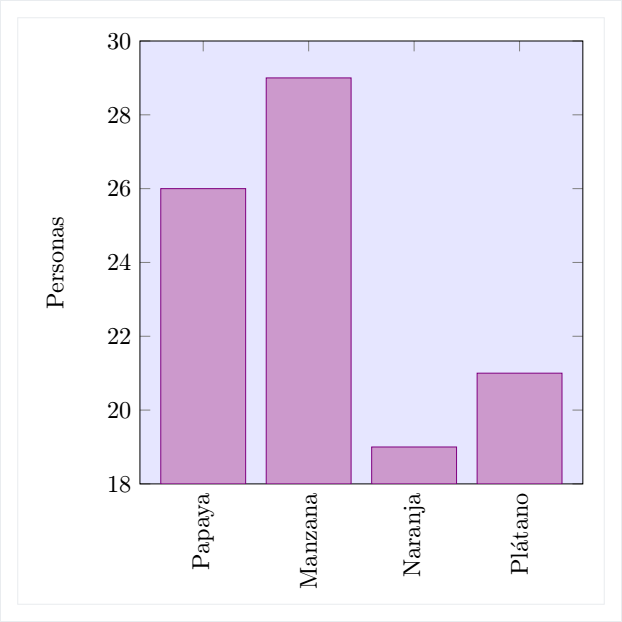
\includegraphics[width=\linewidth]{../images/imagen_barras_frutas01.png}
	% 		\end{parts}
	% 	\end{multicols}

	% }

	\question[2]{Los resultados de una encuesta se muestran en la siguiente gráfica de barras:

		\begin{multicols}{2}
			\begin{parts}\normalsize
				\part ¿Cuántas personas participaron en la encuesta? \fillin[70][1.5cm]
				\part  ¿Cuál es la fruta menos preferida por las personas? \fillin[papaya][1.5cm]
				\part  ¿Cuál es la fruta preferida por las personas? \fillin[plátano][1.5cm]
				\part ¿Cuántas personas prefieren a las \textit{manzanas}.\fillin[16][1.5cm]
				\part ¿Cuántas personas prefieren a los \textit{plátanos}.\fillin[21][1.5cm]
				\part ¿Cuántas personas prefieren a las \textit{naranjas}.\fillin[19][1.5cm]

				\columnbreak%

				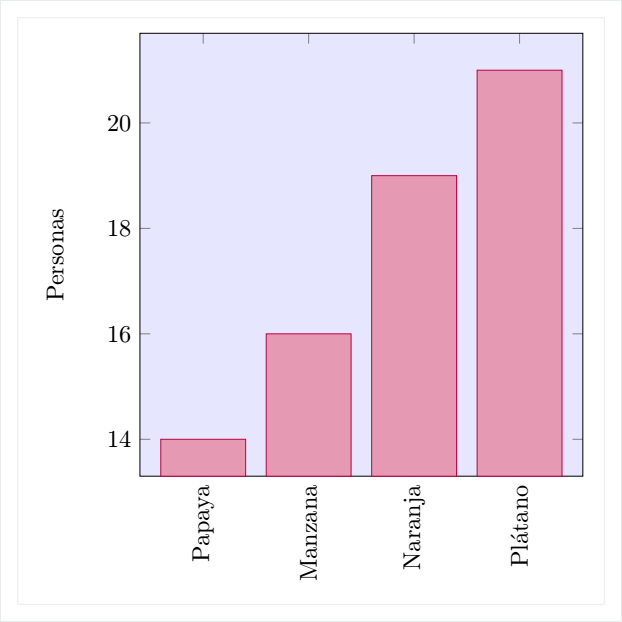
\includegraphics[width=\linewidth]{../images/imagen_barras_frutas02.png}
			\end{parts}
		\end{multicols}
	}

	%%% \addcontentsline{toc}{subsubsection}{Gráficas circulares}
	%%% \subsubsection*{Gráficas circulares}

	\question[2]{Los resultados de una encuesta se muestran en la siguiente gráfica de barras:

		\begin{multicols}{2}
			\begin{parts}\normalsize
				\part ¿Cuántas personas participaron en la encuesta? \fillin[140][1.5cm]
				\part  ¿Cuál es la fruta menos preferida por las personas? \fillin[uva][1.5cm]
				\part  ¿Cuál es la fruta preferida por las personas? \fillin[manzana][1.5cm]
				\part ¿Cuántas personas prefieren a las \textit{manzanas}.\fillin[40][1.5cm]
				\part ¿Cuántas personas prefieren a las \textit{uvas}.\fillin[28][1.5cm]
				\part ¿Cuántas personas prefieren a las \textit{naranjas}.\fillin[35][1.5cm]

				\columnbreak%

				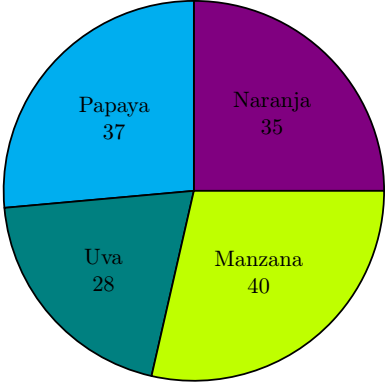
\includegraphics[width=0.8\linewidth]{../images/imagen_pie_frutas01.png}
			\end{parts}
		\end{multicols}

	}

	\newpage

	% \addcontentsline{toc}{subsubsection}{Probabilidad}
	% \subsubsection*{Probabilidad}
	\question[2]{Resuelve los siguientes problemas:

	\begin{multicols}{2}

		\begin{parts}
			% \part En una urna hay 10 pelotas azules, 5 verdes, 15 blancas y 20 negras. Calcula la probabilidad de sacar una pelota negra.

			% \begin{solutionbox}{1.5cm}
			% \end{solutionbox}

			\part Si se lanzan tres monedas al aire, calcula la probabilidad de que caiga puro sol.

			\begin{solutionbox}{2cm}
			\end{solutionbox}

			\part En una urna hay 8 pelotas moradas, 12 naranjas, 7 rojas, 11 azules y 7 blancas. Calcula la probabilidad de sacar una pelota negra.

			\begin{solutionbox}{1.5cm}
			\end{solutionbox}
		\end{parts}
	\end{multicols}
	}

	\addcontentsline{toc}{subsection}{Razones y proporciones}
	\subsection*{Razones y proporciones}
	%%% \addcontentsline{toc}{subsubsection}{Razones 1}
	%%% \subsubsection*{Razones 1}
	%%% \addcontentsline{toc}{subsubsection}{Razones 2}
	%%% \subsubsection*{Razones 2}

	\question[2]{Resuelve los siguientes problemas:

		\begin{multicols}{2}
			\begin{parts}
				\part El perímetro de una cancha de fútbol mide 432 metros. Si la razón entre el ancho y el largo es de 5:7, ¿cuánto mide el largo de la cancha? \hfill\fillin[126][2cm]
				% \part En un salón, la razón entre la cantidad de mujeres y hombres es 7:8. Si hay un total de 45 alumnos entre hombres y mujeres, ¿cuántos son hombres? \hfill\fillin[21][2cm]
				% \part En un salón, la razón entre la cantidad de hombres y mujeres es 3:2. Si hay un total de 40 alumnos entre hombres y mujeres, ¿cuántos hombres hay? \hfill\fillin[24][2cm]
				\part Un fontanero y su ayudante reciben la cantidad de 2700 pesos por la instalación de equipo sanitario, si se reparten el dinero en razón de 7:2 respectivamente, ¿cuánto dinero recibirá el ayudante? \hfill\fillin[600][2cm]
				% \part El perímetro de una cancha de fútbol mide 533 metros. Si la razón entre el ancho y el largo es de 6:7, ¿cuánto mide el ancho de la cancha? \hfill\fillin[123][2cm]
			\end{parts}
		\end{multicols}
	}


	%%% \addcontentsline{toc}{subsubsection}{Encontrando el valor de x}
	%%% \subsubsection*{Encontrando el valor de x}

	\question[2]{Calcula el valor de $x$ en las siguientes proporciones:

		\begin{multicols}{2}
			\begin{parts}
				% \part $ 2.6:7.8=3:x$ \fillin[$9$][1cm]
				\part $ x:4=15:6$ \fillin[$10$][1cm]
				\part $ 7.4:x=3.7:0.5$ \fillin[$1$][1cm]
				\part $ 49:56=x:8$ \fillin[$7$][1cm]
				\part $ 8:3.2=7.5:x$ \fillin[$3$][1cm]
			\end{parts}
		\end{multicols}
	}


	%%% \addcontentsline{toc}{subsubsection}{Proporción directa}
	%%% \subsubsection*{Proporción directa}
		%%% \addcontentsline{toc}{subsubsection}{Proporción inversa}
	%%% \subsubsection*{Proporción inversa}

	\question[2]{Resuelve los siguientes problemas:

		\begin{multicols}{2}
			\begin{parts}
				% \part Una máquina fabrica 400 tornillos en 5 horas, ¿cuánto tardará en fabricar 1,200 tornillos?
				% \fillin[$15$][1cm]

				% \part Un grifo tiene un caudal de salida de 18 litros por minuto y tarda 14 horas en llenar un tanque. ¿Cuánto tardaría si el caudal fuera de 7 litros por minuto?
				% \fillin[$36$][1cm]

				% \part Por 3 horas de trabajo Alberto ha cobrado 420 pesos. ¿Cuánto cobrará por 8 horas?
				% \fillin[$1120$][1cm]

				\part Un tinaco con 3 grifos tarda en llenarse 24 horas, ¿cuánto tardará en llenarse con 4 grifos?
				\fillin[$18$][1cm]

				% \part Un camión que viaja a 60 kilómetros por hora tarda 40 minutos en cubrir cierto recorrido, ¿cuánto tardará un coche que viaja a 150 kilómetros por hora?
				% \fillin[$16$][1cm]

				% \part Si 12 vacas se comen un granero lleno de paja en 80 días, ¿cuánto tardarán en comerse la misma cantidad de paja 30 vacas?
				% \fillin[$32$][1cm]

				% \part Una sandía cuesta 30 pesos, si Juan ha comprado 6 sandías, ¿cuánto ha pagado en total Juan?
				% \fillin[$180$][1cm]

				\part Diez pintores tardan 16 días en pintar una casa, ¿cuánto tiempo tardarán en hacerlo 8 pintores?
				\fillin[$20$][1cm]

				% \part Un corredor de maratón ha avanzado 2.4 kilómetros en 8 minutos. Si mantiene su velocidad constante, ¿cuánto tardará en completar los 42 kilómetros del maratón?
				% \fillin[$140$][1cm]
			\end{parts}
		\end{multicols}
	}


	\addcontentsline{toc}{subsection}{Círculo}
	\subsection*{Círculo}
	% \addcontentsline{toc}{subsubsection}{Diámetro de un círculo}
	% \subsubsection*{Diámetro de un círculo}
	% \addcontentsline{toc}{subsubsection}{Radio de un círculo}
	% \subsubsection*{Radio de un círculo}

	\question[2]{Contesta las siguientes preguntas:

		\begin{multicols}{2}
			\begin{parts}
				\part ¿Cuál es el diámetro de un círculo que tiene un radio de 21.98?

				\begin{solutionbox}{1.2cm}
					\fillin[43.96][0cm]
				\end{solutionbox}

				\part ¿Cuál es el diámetro de un círculo que tiene un radio de 39.21?

				\begin{solutionbox}{1.2cm}
					\fillin[78.42][0cm]
				\end{solutionbox}

				% \part ¿Cuál es el diámetro de un círculo que tiene un radio de 6.7?

				% \begin{solutionbox}{1cm}
				% 	\fillin[13.4][0cm]
				% \end{solutionbox}

				% \part ¿Cuál es el radio de un círculo que tiene un diámetro de 88.28?

				% \begin{solutionbox}{1cm}
				% 	\fillin[44.19][0cm]
				% \end{solutionbox}

			\end{parts}
		\end{multicols}
	}

	% \addcontentsline{toc}{subsubsection}{Perímetro}
	% \subsubsection*{Perímetro}
	% \addcontentsline{toc}{subsubsection}{Área}
	% \subsubsection*{Área}
\newpage
	\question[2]{Calcula el perímetro y área de los siguientes círculos:

		\begin{multicols}{2}
			\begin{parts}

				% \part 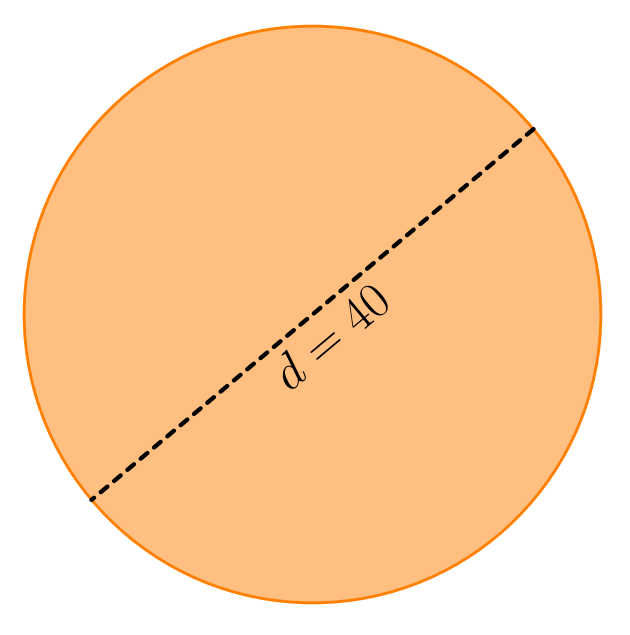
\includegraphics[width=0.7\linewidth]{../images/circulo01.png}\\
				% \normalsize Perímetro: \fillin[62.8][0.3in]  Área: \fillin[1256][0.3in]

				% \begin{solutionbox}{1.2cm}
				% 	% $P=8\pi=8(3.14)=25.12$ \\
				% 	% $A=\pi(4)^2=3.14(4)^2=50.24$
				% \end{solutionbox}

				% \part 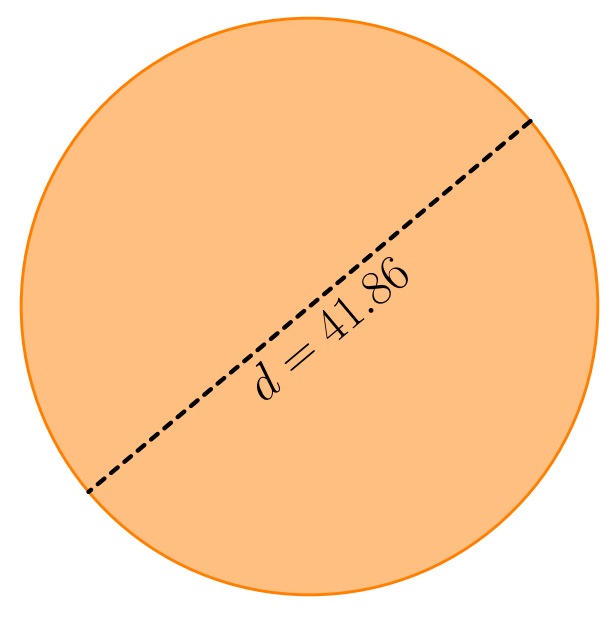
\includegraphics[width=0.7\linewidth]{../images/circulo02.png}\\
				% \normalsize Perímetro: \fillin[131.51][0.3in]  Área: \fillin[1376.22][0.3in]

				% \begin{solutionbox}{1.2cm}
				% 	% $P=2\pi r=2(3.14)(9.3)=58.4$ \\
				% 	% $A=\pi r^2=3.14(9.3)^2=271.57$
				% \end{solutionbox}

				\part 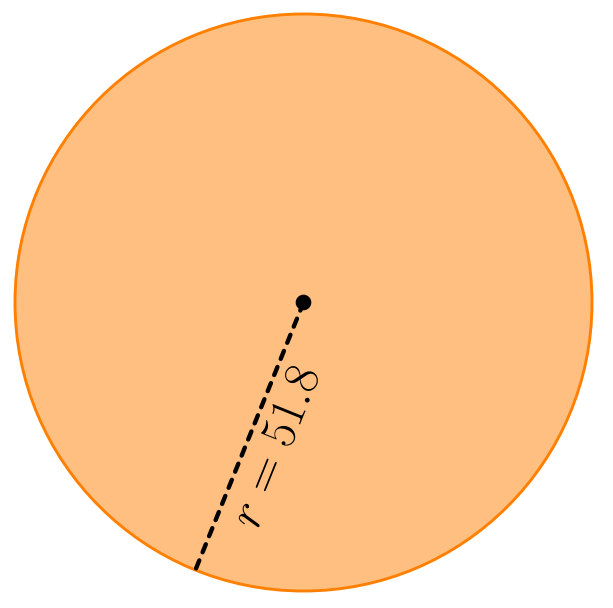
\includegraphics[width=0.55\linewidth]{../images/circulo03.png}\\
				\normalsize Perímetro: \fillin[325.47][0.3in]  Área: \fillin[8429.65][0.3in]

				\begin{solutionbox}{1.2cm}
					% $P=2\pi r=2(3.14)(12)=75.36$ \\
					% $A=\pi r^2=3.14(12)^2=452.16$
				\end{solutionbox}

				\part 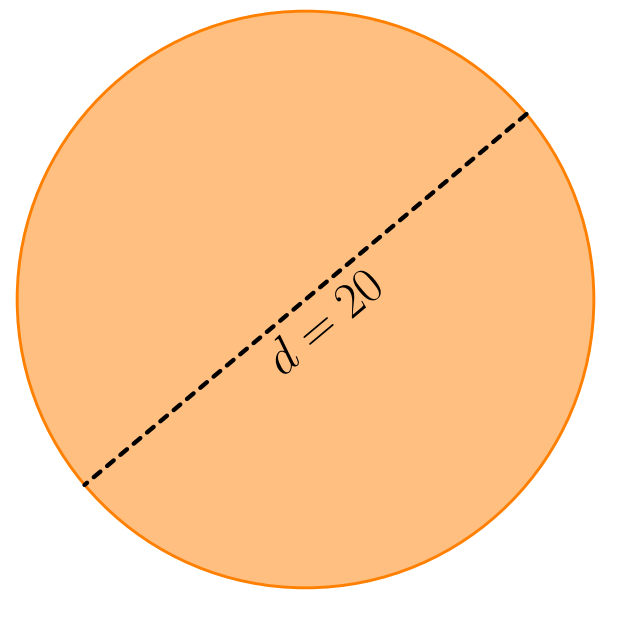
\includegraphics[width=0.55\linewidth]{../images/circulo04.png}\\
				\normalsize Perímetro: \fillin[62.8][0.3in]  Área: \fillin[314][0.3in]

				\begin{solutionbox}{1.2cm}
					% $P=8\pi=8(3.14)=25.12$ \\
					% $A=\pi(4)^2=3.14(4)^2=50.24$
				\end{solutionbox}

				% \part 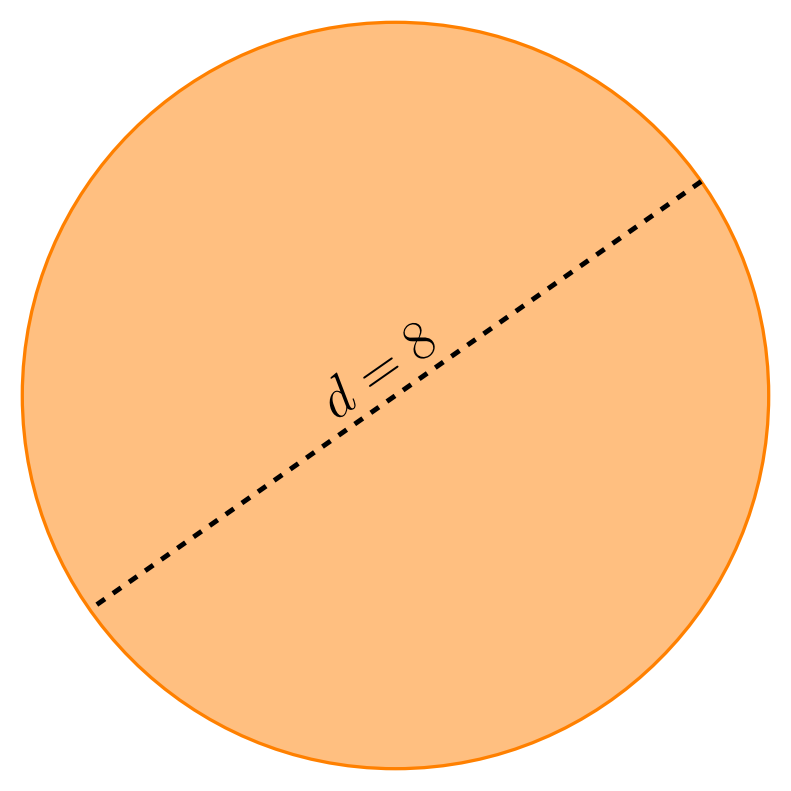
\includegraphics[width=0.7\linewidth]{../images/circulo05.png}\\
				% \normalsize Perímetro: \fillin[25.12][0.3in]  Área: \fillin[50.24][0.3in]

				% \begin{solutionbox}{1.2cm}
				% 	% $P=2\pi r=2(3.14)(9.3)=58.4$ \\
				% 	% $A=\pi r^2=3.14(9.3)^2=271.57$
				% \end{solutionbox}

				% \part 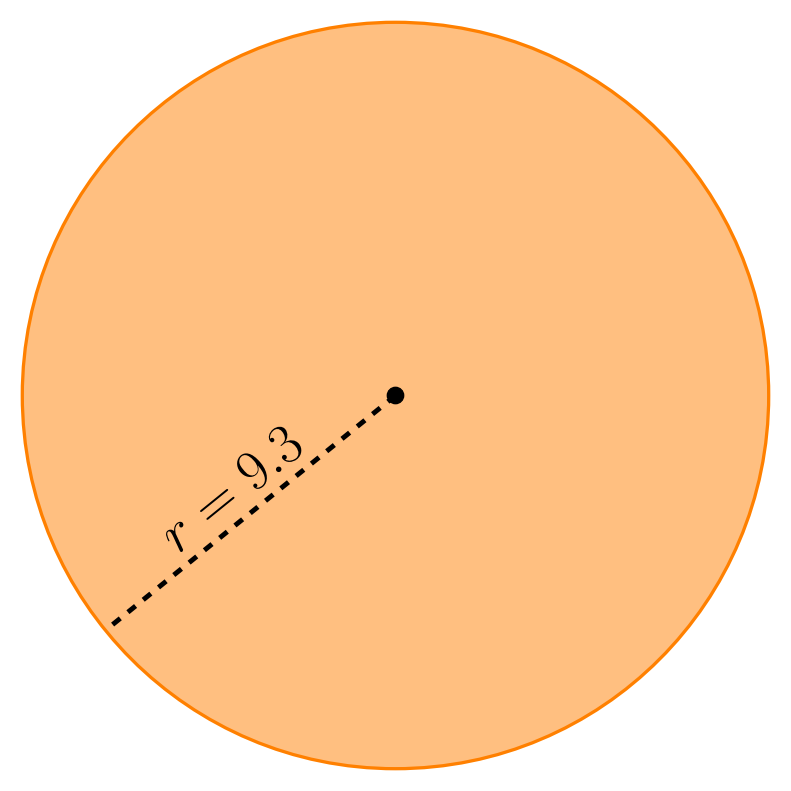
\includegraphics[width=0.7\linewidth]{../images/circulo06.png}\\
				% \normalsize Perímetro: \fillin[58.404][0.3in] Área: \fillin[271.57][0.3in]

				% \begin{solutionbox}{1.2cm}
				% 	% $P=2\pi r=2(3.14)(12)=75.36$ \\
				% 	% $A=\pi r^2=3.14(12)^2=452.16$
				% \end{solutionbox}
			\end{parts}
		\end{multicols}
	}

	% \addcontentsline{toc}{subsubsection}{Resolución de problemas}
	% \subsubsection*{Resolución de problemas}

	\addcontentsline{toc}{subsection}{Figuras geométricas}
	\subsection*{Figuras geométricas}
	% \addcontentsline{toc}{subsubsection}{Nombre de figuras}
	% \subsubsection*{Nombre de figuras}

	\question[2]{Escribe sobre la línea el nombre que recibe cada figura geométrica de acuerdo con su número de lados:

		\begin{multicols}{4}
			\begin{parts}
				\part 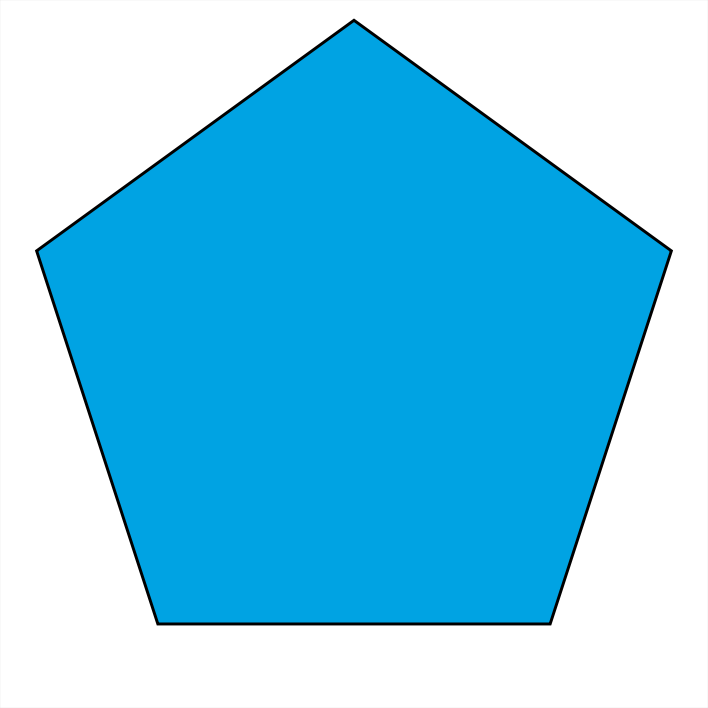
\includegraphics[width=75px]{../images/pentagono_azul.png}  \fillin[pentágono][0.75in]
				\part 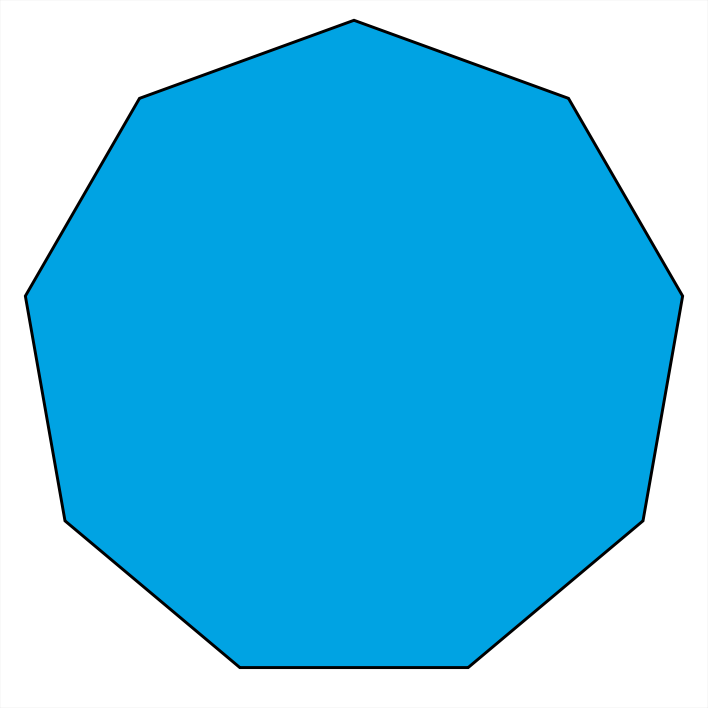
\includegraphics[width=75px]{../images/nonagono_azul.png}   \fillin[nonágono][0.75in]
				\part 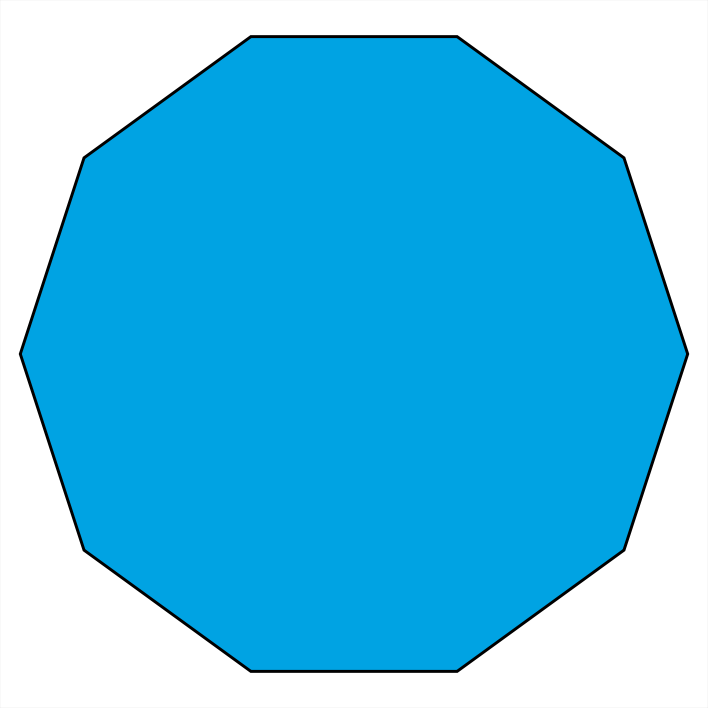
\includegraphics[width=75px]{../images/decagono_azul.png}   \fillin[decágono][0.75in]
				\part 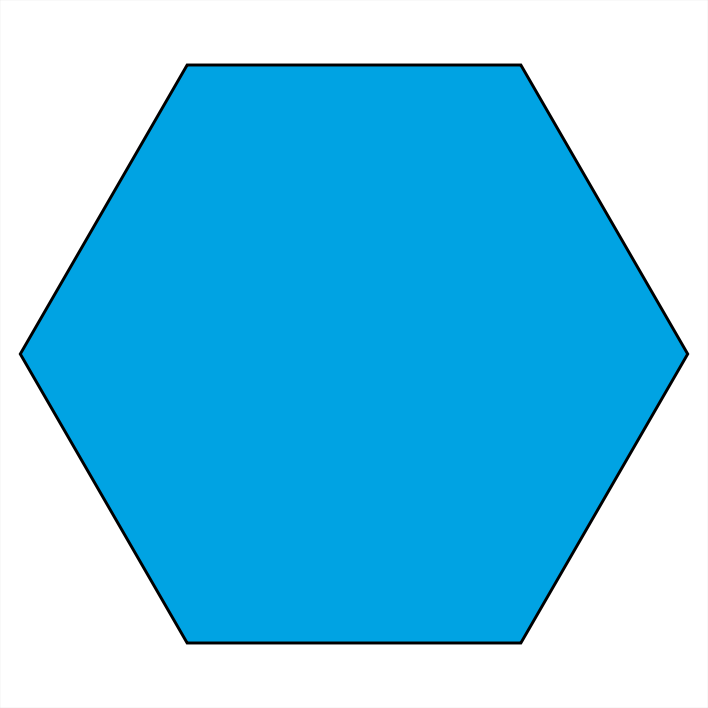
\includegraphics[width=75px]{../images/hexagono_azul.png}   \fillin[hexágono][0.75in]
				% \part 
\includegraphics[width=75px]{../images/rectangulo_azul.png} \fillin[rectángulo][0.75in]
				% \part \includegraphics[width=75px]{../images/cuadrado_azul.png}   \fillin[cuadrado][0.75in]
			\end{parts}
		\end{multicols}
	}

	%%% \addcontentsline{toc}{subsubsection}{Elementos de figuras}
	%%% \subsubsection*{Elementos de figuras}


	% \addcontentsline{toc}{subsubsection}{Perímetro}
	% \subsubsection*{Perímetro}

	\question[2]{Contesta las preguntas sobre perímetros y áreas de figuras geométricas

		\begin{multicols}{2}
			\begin{parts}
				% \part ¿Cuál es el perímetro de un rectángulo cuya base mide 38 y su altura mide 19?

				% \begin{solutionbox}{1cm}
				% 	\[P=38+19+38+19=\color{red}114\]
				% \end{solutionbox}

				% \part ¿Cuál es el perímetro de un cuadrado que sus lados miden 5?

				% \begin{solutionbox}{1cm}
				% 	\[P=5+5+5+5=\color{red}20\]
				% \end{solutionbox}

				\part ¿Cuál es el perímetro de un pentágono que sus lados miden 18?

				\begin{solutionbox}{1.5cm}
					\[P=18 \times 5=\color{red}90\]
				\end{solutionbox}

				% \part ¿Cuál es el perímetro de un octágono que sus lados miden 15?

				% \begin{solutionbox}{1cm}
				% 	\[P=15 \times 8=\color{red}120\]
				% \end{solutionbox}

				% \part ¿Cuál es el perímetro de un rombo que sus lados miden 16?

				% \begin{solutionbox}{1cm}
				% 	\[P=16 \times 4=\color{red}64\]
				% \end{solutionbox}

				\part ¿Cuál es el área de un triángulo cuya base mide 18 y su altura mide 11?

				\begin{solutionbox}{1.5cm}
					\[A=\dfrac{18 \times 11}{2}=\color{red}99\]
				\end{solutionbox}
			\end{parts}
		\end{multicols}
	}

	% \addcontentsline{toc}{subsubsection}{Área}
	% \subsubsection*{Área}

	% \question[2]{Contesta las preguntas sobre áreas de figuras geométricas

	% 	\begin{multicols}{2}
	% 		\begin{parts}
	% 			\part ¿Cuál es el área de un triángulo cuya base mide 18 y su altura mide 11?

	% 			\begin{solutionbox}{1.5cm}
	% 				\[A=\dfrac{18 \times 11}{2}=\color{red}99\]
	% 			\end{solutionbox}


	% 			\part ¿Cuál es el área de un cuadrado que sus lados miden 29?

	% 			\begin{solutionbox}{1.5cm}
	% 				\[A=29 \times 29=\color{red}841\]
	% 			\end{solutionbox}

	% 		\end{parts}
	% 	\end{multicols}
	% }

	% \addcontentsline{toc}{subsubsection}{Resolución de problemas}
	% \subsubsection*{Resolución de problemas}

	\question[2]{Resuelve los siguientes problemas:

		\begin{multicols}{2}
			\begin{parts}
				% \part Alejandro quiere poner una barda alrededor de un terreno cuadrangular que mide 22 metros por lado. ¿Cuánta barda necesitará Alejandro para poner barda en todo el terreno?

				% \begin{solutionbox}{1cm}
				% 	\fillin[88][0in]
				% \end{solutionbox}

				\part Para darle mantenimiento a una alberca olímpica se pone cinta alrededor de esta. Si la alberca tiene 50 metros de largo y 25 metros de ancho, ¿cuánta cinta se necesita para darle la vuelta a la alberca?

				\begin{solutionbox}{1.5cm}
					\fillin[150][0in]
				\end{solutionbox}


				% \part Bruno corre todos los días en un parque de forma rectangular el cual mide 75 metros de largo y 40 metros de ancho. ¿Cuántos metros corre Bruno por una vuelta?

				% \begin{solutionbox}{1cm}
				% 	\fillin[230][0in]
				% \end{solutionbox}

				\part Bruno corre todos los días en un parque de forma rectangular el cual mide 50 metros de largo y 28 metros de ancho. Si al día le da 4 vueltas al parque, ¿cuántos metros habrá corrido en total Bruno?

				\begin{solutionbox}{1.5cm}
					\fillin[624][0in]
				\end{solutionbox}
			\end{parts}
		\end{multicols}
	}

	\addcontentsline{toc}{subsection}{Cuerpos geométricos}
	\subsection*{Cuerpos geométricos}
	%%% \addcontentsline{toc}{subsubsection}{Nombre de cuerpos geométricos}
	%%% \subsubsection*{Nombre de cuerpos geométricos}
	%%% \addcontentsline{toc}{subsubsection}{Elementos de cuerpos geométricos}
	%%% \subsubsection*{Elementos de cuerpos geométricos}
	%%% \addcontentsline{toc}{subsubsection}{Área lateral}
	%%% \subsubsection*{Área lateral}
	%%% \addcontentsline{toc}{subsubsection}{Área total}
	%%% \subsubsection*{Área total}
	%%% \addcontentsline{toc}{subsubsection}{Volumen}
	%%% \subsubsection*{Volumen}

	\question[4]{Calcula el volumen, el área lateral y el área total de las siguientes figuras:
    
	\begin{multicols}{2}
            \begin{parts}
                % \part 
				% \includegraphics[width=0.6\linewidth]{mex_0025.png}\\
                % Prisma cuyos lados "l" de la base miden 8 cm y la altura "h" mide 21 cm.\\
                % Volumen: \fillin[u$^3$][0.4in] \\A. Lateral: \fillin[][0.4in] \\ A. Total: \fillin[u$^2$][0.4in]

                % \part \includegraphics[width=\linewidth]{mex_0023.png}
                % Pirámide cuyos lados "l" de la base miden 13 cm y la altura "h" mide 42 cm.\\
                % Volumen: \fillin[$$ u$^3$][0.4in] \\A. Lateral: \fillin[$$ u][0.4in] \\ A. Total: \fillin[$$ u$^2$][0.4in]

                \part 
				\includegraphics[width=0.6\linewidth]{mex_0024.png}\\
                Cilindro con altura $h=17$ cm y un radio $r=4$ cm.\\
              \small  Volumen: \fillin[u$^3$][0.4in] \\A. Lateral: \fillin[][0.4in] \\ A. Total: \fillin[u$^2$][0.4in]

                % \part \includegraphics[width=\linewidth]{mex_0025.png}
                % Volumen: \fillin[$$ u$^3$][0.4in] \\A. Lateral: \fillin[$$ u][0.4in] \\ A. Total: \fillin[$$ u$^2$][0.4in]

                \part \includegraphics[width=0.6\linewidth]{mex_0026.png}\\
                Prisma cuyos lados "l" de la base miden 15 cm y la altura "h" mide 24 cm.\\
               \small Volumen: \fillin[u$^3$][0.4in] \\A. Lateral: \fillin[][0.4in] \\ A. Total: \fillin[u$^2$][0.4in]

                \part 
				\includegraphics[width=0.6\linewidth]{mex_0027.png}\\
                Pirámide de 19 cm de altura cuya base es un pentágono cuyos lados "l" miden 8 cm y su apotema "a" mide 5 cm.\\
              \small  Volumen: \fillin[u$^3$][0.4in] \\A. Lateral: \fillin[][0.4in] \\ A. Total: \fillin[u$^2$][0.4in]

                % \part \includegraphics[width=\linewidth]{mex_0028.png}
                % Volumen: \fillin[$$ u$^3$][0.4in] \\A. Lateral: \fillin[$$ u][0.4in] \\ A. Total: \fillin[$$ u$^2$][0.4in]

                \part 
				\includegraphics[width=0.6\linewidth]{mex_0029.png}\\
                Pirámide cuyos lados "l" de la base miden 16 cm y la altura "h" mide 27 cm.\\
               \small Volumen: \fillin[u$^3$][0.4in] \\A. Lateral: \fillin[][0.4in] \\ A. Total: \fillin[u$^2$][0.4in]

                % \part \includegraphics[width=\linewidth]{mex_0030.png}
                % Volumen: \fillin[$$ u$^3$][0.4in] \\A. Lateral: \fillin[$$ u][0.4in] \\ A. Total: \fillin[$$ u$^2$][0.4in]
            \end{parts}
        \end{multicols}
    }


	\addcontentsline{toc}{subsection}{Sistema de unidades}
	\subsection*{Sistema de unidades}
	% \addcontentsline{toc}{subsubsection}{Operaciones con múltiplos de 10}
	% \subsubsection*{Operaciones con múltiplos de 10}

	\question[4]{Realiza las siguientes operaciones:

		\begin{multicols}{3}
			\begin{parts}
				% \part $ 93.2 \times 1000=$   \fillin[93200][0.5in]
				% \part $ 84.2 \times 100=$   \fillin[8420][0.5in]
				\part $ 66.472 \times 10000=$   \fillin[664720][0.5in]
				% \part $ 192.3 \times 10=$   \fillin[1923][0.5in]
				\part $ 26.9 \times 1000=$   \fillin[26900][0.5in]
				\part $ 81.674 \times 100000=$   \fillin[8167400][0.5in]
				\part $ 1.2 \times 1000=$   \fillin[1200][0.5in]
				% \part $ 7.8 \times 10=$   \fillin[78][0.5in]
				% \part $ 38093 \divisionsymbol 10=$   \fillin[3809.3][0.5in]
				\part $ 28 \divisionsymbol 1000=$   \fillin[0.028][0.5in]
				% \part $ 44567 \divisionsymbol 100=$   \fillin[445.67][0.5in]
				% \part $ 678 \divisionsymbol 1000=$   \fillin[0.678][0.5in]
				\part $ 7.1 \divisionsymbol 10=$   \fillin[0.71][0.5in]
				% \part $ 51 \divisionsymbol 100=$   \fillin[0.51][0.5in]
				% \part $ 3.9 \divisionsymbol 100=$   \fillin[0.039][0.5in]
				% \part $ 2.4 \divisionsymbol 100=$   \fillin[0.024][0.5in]
				% \part $ 34 \divisionsymbol 10=$   \fillin[3.4][0.5in]
				% \part $ 6.3 \divisionsymbol 10000=$   \fillin[0.00063][0.5in]
			\end{parts}
		\end{multicols}
	}

	% \addcontentsline{toc}{subsubsection}{Unidades de longitud}
	% \subsubsection*{Unidades de longitud}
	% \addcontentsline{toc}{subsubsection}{Unidades de masa}
	% \subsubsection*{Unidades de masa}
	% \addcontentsline{toc}{subsubsection}{Unidades de capacidad}
	% \subsubsection*{Unidades de capacidad}
	% \addcontentsline{toc}{subsubsection}{Unidades de área y volumen}
	% \subsubsection*{Unidades de área y volumen}
	\question[6]{Realiza las siguientes conversiones de unidades de longitud y masa:

		\begin{multicols}{2}
			\begin{parts}%\normalsize
			% \part De 157 kilómetros a hectómetros. \hfill \fillin[1570][0.6in] hm
				% \part De 25 centímetros a milímetros.  \hfill \fillin[250][0.6in] mm
				% \part De 27 kilómetros a decámetros.   \hfill \fillin[2700][0.6in] Dm
				% \part De 17 kilómetros a hectómetros.  \hfill \fillin[170][0.6in] hm
				%  \part De 69 kilómetros a centímetros.  \hfill \fillin[6900000][0.6in] cm
				\part De 59 decímetros a centímetros.  \hfill \fillin[590][0.6in] cm
				% \part De 26 metros a decímetros.       \hfill \fillin[260][0.6in] dm
				\part De 4 kilómetros a milímetros.    \hfill \fillin[4000000][0.6in] mm
				% \part De 135 kilómetros a decámetros.  \hfill \fillin[13500][0.6in] Dm
				% \part De 112 kilómetros a hectómetros. \hfill \fillin[1120][0.6in] hm
				% \part De 205 gramos a decigramos    \hfill \fillin[2050][0.5in] dg
				% \part De 25 kilogramos a gramos     \hfill \fillin[25000][0.5in] g
				% \part De 58 kilogramos a gramos     \hfill \fillin[58000][0.5in] g
				% \part De 45 decagramos a gramos     \hfill \fillin[450][0.5in] g
				% \part De 134 gramos a decigramos    \hfill \fillin[1340][0.5in] dg
				 \part De 282 gramos a miligramos    \hfill \fillin[282000][0.5in] mg
				% \part De 117 decagramos a gramos    \hfill \fillin[1170][0.5in] g
				% \part De 17 decigramos a miligramos \hfill \fillin[1700][0.5in] mg
				\part De 115 gramos a centigramos   \hfill \fillin[11500][0.5in] cg
				% \part De 62 gramos a miligramos     \hfill \fillin[62000][0.5in] mg
		\part De 8.03 metros cúbicos a milímetros cúbicos 
		\part De 88 metros cuadrados a kilómetros cuadrados
			\end{parts}
		\end{multicols}
	}
\end{questions}
\end{document}